% Options for packages loaded elsewhere
\PassOptionsToPackage{unicode}{hyperref}
\PassOptionsToPackage{hyphens}{url}
%
\documentclass[
]{article}
\usepackage{lmodern}
\usepackage{amssymb,amsmath}
\usepackage{ifxetex,ifluatex}
\ifnum 0\ifxetex 1\fi\ifluatex 1\fi=0 % if pdftex
  \usepackage[T1]{fontenc}
  \usepackage[utf8]{inputenc}
  \usepackage{textcomp} % provide euro and other symbols
\else % if luatex or xetex
  \usepackage{unicode-math}
  \defaultfontfeatures{Scale=MatchLowercase}
  \defaultfontfeatures[\rmfamily]{Ligatures=TeX,Scale=1}
\fi
% Use upquote if available, for straight quotes in verbatim environments
\IfFileExists{upquote.sty}{\usepackage{upquote}}{}
\IfFileExists{microtype.sty}{% use microtype if available
  \usepackage[]{microtype}
  \UseMicrotypeSet[protrusion]{basicmath} % disable protrusion for tt fonts
}{}
\makeatletter
\@ifundefined{KOMAClassName}{% if non-KOMA class
  \IfFileExists{parskip.sty}{%
    \usepackage{parskip}
  }{% else
    \setlength{\parindent}{0pt}
    \setlength{\parskip}{6pt plus 2pt minus 1pt}}
}{% if KOMA class
  \KOMAoptions{parskip=half}}
\makeatother
\usepackage{xcolor}
\IfFileExists{xurl.sty}{\usepackage{xurl}}{} % add URL line breaks if available
\IfFileExists{bookmark.sty}{\usepackage{bookmark}}{\usepackage{hyperref}}
\hypersetup{
  pdftitle={PMD alerts as possible kludges: open, fixed or new?},
  pdfauthor={Bruno Crotman},
  hidelinks,
  pdfcreator={LaTeX via pandoc}}
\urlstyle{same} % disable monospaced font for URLs
\usepackage[margin=1in]{geometry}
\usepackage{color}
\usepackage{fancyvrb}
\newcommand{\VerbBar}{|}
\newcommand{\VERB}{\Verb[commandchars=\\\{\}]}
\DefineVerbatimEnvironment{Highlighting}{Verbatim}{commandchars=\\\{\}}
% Add ',fontsize=\small' for more characters per line
\usepackage{framed}
\definecolor{shadecolor}{RGB}{248,248,248}
\newenvironment{Shaded}{\begin{snugshade}}{\end{snugshade}}
\newcommand{\AlertTok}[1]{\textcolor[rgb]{0.94,0.16,0.16}{#1}}
\newcommand{\AnnotationTok}[1]{\textcolor[rgb]{0.56,0.35,0.01}{\textbf{\textit{#1}}}}
\newcommand{\AttributeTok}[1]{\textcolor[rgb]{0.77,0.63,0.00}{#1}}
\newcommand{\BaseNTok}[1]{\textcolor[rgb]{0.00,0.00,0.81}{#1}}
\newcommand{\BuiltInTok}[1]{#1}
\newcommand{\CharTok}[1]{\textcolor[rgb]{0.31,0.60,0.02}{#1}}
\newcommand{\CommentTok}[1]{\textcolor[rgb]{0.56,0.35,0.01}{\textit{#1}}}
\newcommand{\CommentVarTok}[1]{\textcolor[rgb]{0.56,0.35,0.01}{\textbf{\textit{#1}}}}
\newcommand{\ConstantTok}[1]{\textcolor[rgb]{0.00,0.00,0.00}{#1}}
\newcommand{\ControlFlowTok}[1]{\textcolor[rgb]{0.13,0.29,0.53}{\textbf{#1}}}
\newcommand{\DataTypeTok}[1]{\textcolor[rgb]{0.13,0.29,0.53}{#1}}
\newcommand{\DecValTok}[1]{\textcolor[rgb]{0.00,0.00,0.81}{#1}}
\newcommand{\DocumentationTok}[1]{\textcolor[rgb]{0.56,0.35,0.01}{\textbf{\textit{#1}}}}
\newcommand{\ErrorTok}[1]{\textcolor[rgb]{0.64,0.00,0.00}{\textbf{#1}}}
\newcommand{\ExtensionTok}[1]{#1}
\newcommand{\FloatTok}[1]{\textcolor[rgb]{0.00,0.00,0.81}{#1}}
\newcommand{\FunctionTok}[1]{\textcolor[rgb]{0.00,0.00,0.00}{#1}}
\newcommand{\ImportTok}[1]{#1}
\newcommand{\InformationTok}[1]{\textcolor[rgb]{0.56,0.35,0.01}{\textbf{\textit{#1}}}}
\newcommand{\KeywordTok}[1]{\textcolor[rgb]{0.13,0.29,0.53}{\textbf{#1}}}
\newcommand{\NormalTok}[1]{#1}
\newcommand{\OperatorTok}[1]{\textcolor[rgb]{0.81,0.36,0.00}{\textbf{#1}}}
\newcommand{\OtherTok}[1]{\textcolor[rgb]{0.56,0.35,0.01}{#1}}
\newcommand{\PreprocessorTok}[1]{\textcolor[rgb]{0.56,0.35,0.01}{\textit{#1}}}
\newcommand{\RegionMarkerTok}[1]{#1}
\newcommand{\SpecialCharTok}[1]{\textcolor[rgb]{0.00,0.00,0.00}{#1}}
\newcommand{\SpecialStringTok}[1]{\textcolor[rgb]{0.31,0.60,0.02}{#1}}
\newcommand{\StringTok}[1]{\textcolor[rgb]{0.31,0.60,0.02}{#1}}
\newcommand{\VariableTok}[1]{\textcolor[rgb]{0.00,0.00,0.00}{#1}}
\newcommand{\VerbatimStringTok}[1]{\textcolor[rgb]{0.31,0.60,0.02}{#1}}
\newcommand{\WarningTok}[1]{\textcolor[rgb]{0.56,0.35,0.01}{\textbf{\textit{#1}}}}
\usepackage{graphicx,grffile}
\makeatletter
\def\maxwidth{\ifdim\Gin@nat@width>\linewidth\linewidth\else\Gin@nat@width\fi}
\def\maxheight{\ifdim\Gin@nat@height>\textheight\textheight\else\Gin@nat@height\fi}
\makeatother
% Scale images if necessary, so that they will not overflow the page
% margins by default, and it is still possible to overwrite the defaults
% using explicit options in \includegraphics[width, height, ...]{}
\setkeys{Gin}{width=\maxwidth,height=\maxheight,keepaspectratio}
% Set default figure placement to htbp
\makeatletter
\def\fps@figure{htbp}
\makeatother
\setlength{\emergencystretch}{3em} % prevent overfull lines
\providecommand{\tightlist}{%
  \setlength{\itemsep}{0pt}\setlength{\parskip}{0pt}}
\setcounter{secnumdepth}{5}
\usepackage{lscape}
\newcommand{\blandscape}{\begin{landscape}}
\newcommand{\elandscape}{\end{landscape}}
\definecolor{darkred}{RGB}{150, 40, 40}
\definecolor{darkgreen}{RGB}{30, 120, 30}
\definecolor{darkorange}{RGB}{40, 40, 160}
\usepackage{booktabs}
\usepackage{longtable}
\usepackage{array}
\usepackage{multirow}
\usepackage{wrapfig}
\usepackage{float}
\usepackage{colortbl}
\usepackage{pdflscape}
\usepackage{tabu}
\usepackage{threeparttable}
\usepackage{threeparttablex}
\usepackage[normalem]{ulem}
\usepackage{makecell}
\usepackage{xcolor}

\title{PMD alerts as possible kludges: open, fixed or new?}
\author{Bruno Crotman}
\date{}

\begin{document}
\maketitle

{
\setcounter{tocdepth}{3}
\tableofcontents
}
\small

\normalsize

\section{Introduction}\label{intro}

Agota teste vindo o RStudio This document is part of a larger research project about software
degradation caused by careless developers' behavior and strategies to
deal with such undesired behavior. The strategies to deal with this
problem will possibly be inspired by concepts from game theory. At this
moment, we assume that software degradation can be measured by the
number and the types of kludges made by software developers in the code.
So, one of the goals of this project is to study how software projects
evolve in terms of number and kinds of kludges. Right now, we are trying
to identify kludges by looking at alerts generated by the PMD source
code analyzer.

To evaluate how the number of alerts evolves throughout the history of a
software project, we must be able to analyze two different versions of a
source code (an old and a new version) and categorize each alert
contained in the new version as either \textbf{new}, \textbf{fixed} or
\textbf{open}.

A PMD alert generated for the old version is either \textbf{open} or
\textbf{fixed} in the new version. An \textbf{open} alert remains in the
new version of the code. A \textbf{fixed} alert does not exist in the
new version.

A PMD alert generated for the new version is either \textbf{open} or
\textbf{new}. An \textbf{open} alert indicates that the same alert was
identified in the old version. A \textbf{new} alert implies that the
same alert cannot be identified in the old version.

The alerts identified as \textbf{open} are equivalent in both new and
old versions. To decide whether an alert is \textbf{open},
\textbf{fixed} or \textbf{new}, one has to identify if an alert in the
old version is equivalent to an alert in the new version. The
intersection between \textbf{fixed} alerts, \textbf{new} alerts and
\textbf{open} alerts is empty.

In order to decide if an alert is \textbf{open}, \textbf{fixed} or
\textbf{new}, we have to identify if an alert in the old version is
equivalent to an alert in the new version. This document describes the
algorithms we are using to make this classification.

In Section \ref{pmd}, we describe how we use PMD source code analyzer in
two tasks:

\begin{itemize}
\item The first task is to list the alerts that represent possible kludges. 
PMD receives a source code as input and generates a list of bad programming practices contained in the code, i.e., the alerts. 
The process we follow to generate the alerts using PMD source code analyzer is discussed in Section \ref{pmd_alerts}. 
\item The second task for which we use PMD is in the creation of an Abstract Syntax Tree (AST) from a source code, with selected nodes. 
This will help us in the algorithm described in Section \ref{alg2}. 
The creation of the AST using PMD is described in Section \ref{ast}.
\end{itemize}

In Section \ref{alg}, we describe two algorithms that help to categorize
the alerts as \textbf{new}, \textbf{fixed} or \textbf{open}. The first
one, described in Section \ref{alg1}, is a naive algorithm based on
matches by lines of code and some key features of the alerts. The second
is a more sophisticated algorithm, based on matches by blocks of code,
using the Abstract Syntax Tree.

\section{PMD Source Code Analyzer}\label{pmd}

PMD is static source code analyzer that is commonly used to find
possible programming flaws. In this work we use PMD for two tasks: to
generate alerts that we interpret as clues about kludges and to create
an AST from the source code with selected kinds of node.

\subsection{Using PMD to generate alerts}\label{pmd_alerts}

PMD traverses the AST of a source code searching for violations of rules
which are configured by the user. PMD comes with a default rule set for
Java language. The default rule set finds common programming flaws like
unused variables, empty catch blocks, unnecessary object creation, and
so forth. It´s possible to configure a different set of rules creating a
custom XML file. At this point we use the default rule set to generate
the alerts that we interpret as kludges and try to categorize by the
algorithms described in Section \ref{alg}

\newpage

In Figure \ref{simple_code}, we can see an example of a simple code and
the alerts that were generated by the default rule set of PMD alerts
tool.

\small

\begin{verbatim}
## [1] "file"
## little-tree_little-tree-new.diff
\end{verbatim}

\normalsize

\small

\begin{Shaded}
\begin{Highlighting}[]
\CommentTok{/*  1-                                   */}\KeywordTok{package}\ImportTok{ pack_x;}
\CommentTok{/*  2-                                   */}  
\CommentTok{/*  3-                                   */}\KeywordTok{import}\ImportTok{ importX.function;}
\CommentTok{/*  4-                                   */}
\CommentTok{/*  5-                                   */}\KeywordTok{class}\NormalTok{ ClassX }\KeywordTok{extends}\NormalTok{ ClassY }\KeywordTok{implements}\NormalTok{ InterfX \{}
\CommentTok{/*  6-                                   */}    \KeywordTok{private} \DataTypeTok{long}\NormalTok{ fieldX;}
\CommentTok{/*  7-                                   */}    
\CommentTok{/*  8-                                   */}    \FunctionTok{ClassX}\NormalTok{(}\DataTypeTok{int}\NormalTok{ paramX, }\DataTypeTok{double}\NormalTok{ paramY) \{      }
\CommentTok{/*  9-                                   */}        \DataTypeTok{int}\NormalTok{ varX = }\FunctionTok{function}\NormalTok{(paramX, paramY);     }
\CommentTok{/* 10-                                   */}        \KeywordTok{if}\NormalTok{ (varX == }\DecValTok{0}\NormalTok{)}
\CommentTok{/* 11-ControlStatementBraces             */}            \KeywordTok{this}\NormalTok{.}\FunctionTok{fieldX}\NormalTok{ = }\DecValTok{1}\NormalTok{;}
\CommentTok{/* 12-                                   */}        \KeywordTok{else}\NormalTok{\{}
\CommentTok{/* 13-                                   */}            \KeywordTok{this}\NormalTok{.}\FunctionTok{fieldX}\NormalTok{ = }\DecValTok{0}\NormalTok{;}
\CommentTok{/* 14-                                   */}\NormalTok{     \}}
\CommentTok{/* 15-                                   */}\NormalTok{    \}}
\CommentTok{/* 16-                                   */}    \AttributeTok{@Override}
\CommentTok{/* 17-                                   */}    \KeywordTok{public} \DataTypeTok{int} \FunctionTok{methodX}\NormalTok{(}\DataTypeTok{int}\NormalTok{ paramW, }\BuiltInTok{Boolean}\NormalTok{ paramZ)}
\CommentTok{/* 18-                                   */}\NormalTok{    \{}
\CommentTok{/* 19-                                   */}        \KeywordTok{if}\NormalTok{ (paramZ)}
\CommentTok{/* 20-ControlStatementBraces             */}\NormalTok{            fieldX = paramW;}
\CommentTok{/* 21-                                   */}        \KeywordTok{else}\NormalTok{\{}
\CommentTok{/* 22-                                   */}\NormalTok{            fieldX = }\DecValTok{0}\NormalTok{;}
\CommentTok{/* 23-                                   */}\NormalTok{     \}}
\CommentTok{/* 24-                                   */}        \KeywordTok{return}\NormalTok{ paramW + }\KeywordTok{this}\NormalTok{.}\FunctionTok{fieldX}\NormalTok{;}
\CommentTok{/* 25-                                   */}\NormalTok{     \}}
\CommentTok{/* 26-                                   */}\NormalTok{\}  }
\end{Highlighting}
\end{Shaded}

\normalsize

\begin{figure}
\centering

\includegraphics{figures/fake.png}
\caption{Simple code with its alerts \label{simple_code}}
\end{figure}

\subsection{Using PMD to generate an Abstract Syntax Tree }\label{ast}

The AST is used, in conjunction with the relation between the lines we
will see in Section \ref{map}, to understand the location of an alert in
a version of a code. We use this information in the algorithm described
in Section \ref{alg2}

We can see that the tool traverses the source code visiting many
different kinds of elements. If we build our own simple rules, aimed
only to capture some kinds of elements, we will generate list of
``alerts'' that will contain all the elements of the chosen kinds
contained in the AST.

\newpage

We don´t use all the types of nodes recognized by PMD Alert to generate
the AST. The kinds of elements that were selected are the following
ones:

\begin{itemize}
\item \textbf{Annotation}: a syntatic metadata added to a source code.
\item \textbf{Block}: a block of statements enclosed by braces.
\item \textbf{ClassOrInterfaceBody}: the body of an interface or a class, excluding the declaration.
\item \textbf{ClassOrInterfaceDeclaration}: class or interface, including the declaration and the body.
\item \textbf{ClassOrInterfaceType}: declaration of a type.
\item \textbf{CompilationUnit}: the root of an AST tree.
\item \textbf{ConstructorDecaration}: class or interface, including the declaration and the body.
\item \textbf{ExtendsList}: list of extensions of a class.
\item \textbf{FieldDeclaration}: field declaration, including the type, the name and the possible assignment.
\item \textbf{FormalParameter}: a parameter of a method or constructor.
\item \textbf{FormalParameters}:  list of formal parameters of a method or constructor.
\item \textbf{IfStatement}: an if statements including its blocks and condition.
\item \textbf{ImplementsList}: list of implementations of an interface.
\item \textbf{Import}: a package imported.
\item \textbf{Method}: a method, including body and declaration.
\item \textbf{Name}: a named value, like a variable, a class or a package referenced in the code.
\item \textbf{package}: the indication of the package to which the compilation unit belongs.
\item \textbf{statement}: any statement, like an if statement or an assignment.
\item \textbf{TypeDeclaration}: any type declaration.
\item \textbf{VariableId}: the name of a variable in a variable declaration.
\end{itemize}

In order to recreate the AST, we must follow three steps:

\begin{enumerate}
\def\labelenumi{\arabic{enumi}.}
\item
  Link each element \(a\) to the set of elements \(X\) that are fully
  contained between the begin line / begin column and end line / end
  column of element \(a\). We can construct a directed graph in which
  the elements are the nodes and the links described are the edges. This
  is not a tree yet, because each node will have edges directed to all
  its descendants and not only its children in the AST.
\item
  Sort the nodes in the decreasing order of its number of children. The
  objective is to establish that, in a search through this graph, the
  first child chosen will be the one that is a child in the AST, and not
  only a descendant.
\item
  Proceed a deep-first search starting from the compilation unit node.
\end{enumerate}

\section{Algorithms to categorize alerts}\label{alg}

\subsection{Algorithm 1: Matches by line of code}\label{alg1}

In this first algorithm, I match the lines of code of the old version
with the lines of code of the new version using information from the
output of git's diff command. When an alert with the same features
occurs in both matched lines, this alert is declared \textbf{open}. The
alerts that occur in a not matched line of the old version are declared
\emph{fixed} and the alerts located in a unmatched line of the new
version are declared as \textbf{new}.

These are the steps of the algorithm:

\begin{enumerate}
\def\labelenumi{\arabic{enumi}.}
\tightlist
\item
  Generate a list of alerts from each version (old and new) using PMD
  Alert (Section \ref{codes});
\item
  Generate the git diff between the two versions (Section \ref{diff});
\item
  Using information from git diff, create a = map between the lines
  (Section \ref{map});
\item
  Categorize the alerts (Section \ref{categorize}).
\end{enumerate}

\subsubsection{Generate a list of alerts for each version}\label{codes}

\small

\begin{verbatim}
## [1] "file"
## old_original_new_1.diff
\end{verbatim}

\normalsize

The two codes presented in this Section, named ``new version'' and ``old
version'', are used in Sections \ref{diff}, \ref{map} and
\ref{categorize} to describe the algorithm.

The old version, with the alerts generated by PMI, is shown in Figure
\ref{old_example}.

\newpage

\begin{landscape}

\footnotesize

\begin{Shaded}
\begin{Highlighting}[]
\CommentTok{/*  1-                                   */}\KeywordTok{package}\ImportTok{ twitter4j;}
\CommentTok{/*  2-                                   */}
\CommentTok{/*  3-UnusedImports                      */}\KeywordTok{import}\ImportTok{ java.util.concurrent.ConcurrentHashMap;}
\CommentTok{/*  4-                                   */}
\CommentTok{/*  5-                                   */}\KeywordTok{class}\NormalTok{ TwitterImpl }\KeywordTok{extends}\NormalTok{ TwitterBaseImpl }\KeywordTok{implements}\NormalTok{ Twitter \{}
\CommentTok{/*  6-                                   */}    \KeywordTok{private} \DataTypeTok{static} \DataTypeTok{final} \DataTypeTok{long}\NormalTok{ serialVersionUID = }\DecValTok{9170943084096085770L}\NormalTok{;}
\CommentTok{/*  7-UnusedPrivateField                 */}    \KeywordTok{private} \DataTypeTok{static} \DataTypeTok{final} \BuiltInTok{Logger}\NormalTok{ logger = }\BuiltInTok{Logger}\NormalTok{.}\FunctionTok{getLogger}\NormalTok{(TwitterBaseImpl.}\FunctionTok{class}\NormalTok{);}
\CommentTok{/*  8-                                   */}    
\CommentTok{/*  9-                                   */}    \CommentTok{/*package*/}
\CommentTok{/* 10-                                   */}    \FunctionTok{TwitterImpl}\NormalTok{(}\BuiltInTok{Configuration}\NormalTok{ conf, Authorization auth) \{}
\CommentTok{/* 11-                                   *//* ...  */}
\CommentTok{/* 45-                                   *//* ...  */}
\CommentTok{/* 46-                                   */}            \KeywordTok{if}\NormalTok{ (conf.}\FunctionTok{isTweetModeExtended}\NormalTok{()) \{}
\CommentTok{/* 47-                                   */}\NormalTok{                params.}\FunctionTok{add}\NormalTok{(}\KeywordTok{new} \FunctionTok{HttpParameter}\NormalTok{(}\StringTok{"tweet_mode"}\NormalTok{, }\StringTok{"extended"}\NormalTok{));}
\CommentTok{/* 48-                                   */}\NormalTok{            \}}
\CommentTok{/* 49-OptimizableToArrayCall             */}\NormalTok{            HttpParameter[] implicitParams = params.}\FunctionTok{toArray}\NormalTok{(}\KeywordTok{new}\NormalTok{ HttpParameter[params.}\FunctionTok{size}\NormalTok{()]);}
\CommentTok{/* 50-                                   */}
\CommentTok{/* 51-                                   */}            \CommentTok{// implicitParamsMap.containsKey() is evaluated in the above if clause.}
\CommentTok{/* 52-                                   */}            \CommentTok{// thus implicitParamsStrMap needs to be initialized first}
\CommentTok{/* 53-                                   *//* ...  */}
\CommentTok{/* 59-                                   *//* ...  */}
\CommentTok{/* 60-                                   */}
\CommentTok{/* 61-                                   */}    
\CommentTok{/* 62-                                   */}    \AttributeTok{@Override}
\CommentTok{/* 63-FormalParameterNamingConventions   */}    \KeywordTok{public}\NormalTok{ AccountSettings }\FunctionTok{updateAccountSettings}\NormalTok{(}\BuiltInTok{Integer}\NormalTok{ trend_locationWoeid,}
\CommentTok{/* 64-FormalParameterNamingConventions(2)*/}                                                 \BuiltInTok{Boolean}\NormalTok{ sleep_timeEnabled, }\BuiltInTok{String}\NormalTok{ start_sleepTime,}
\CommentTok{/* 65-FormalParameterNamingConventions(2)*/}                                                 \BuiltInTok{String}\NormalTok{ end_sleepTime, }\BuiltInTok{String}\NormalTok{ time_zone, }\BuiltInTok{String}\NormalTok{ lang)}
\CommentTok{/* 66-                                   */}            \KeywordTok{throws}\NormalTok{ TwitterException \{}
\CommentTok{/* 67-                                   */}        \BuiltInTok{List}\NormalTok{<HttpParameter> profile = }\KeywordTok{new} \BuiltInTok{ArrayList}\NormalTok{<HttpParameter>(}\DecValTok{6}\NormalTok{);}
\CommentTok{/* 68-                                   */}        \KeywordTok{if}\NormalTok{ (trend_locationWoeid != }\KeywordTok{null}\NormalTok{) \{}
\CommentTok{/* 69-                                   *//* ...  */}
\CommentTok{/* 83-                                   *//* ...  */}
\CommentTok{/* 84-                                   */}\NormalTok{            profile.}\FunctionTok{add}\NormalTok{(}\KeywordTok{new} \FunctionTok{HttpParameter}\NormalTok{(}\StringTok{"lang"}\NormalTok{, lang));}
\CommentTok{/* 85-                                   */}\NormalTok{        \}}
\CommentTok{/* 86-                                   */}        \KeywordTok{return}\NormalTok{ factory.}\FunctionTok{createAccountSettings}\NormalTok{(}\FunctionTok{post}\NormalTok{(conf.}\FunctionTok{getRestBaseURL}\NormalTok{() + }\StringTok{"account/settings.json"}
\CommentTok{/* 87-OptimizableToArrayCall             */}\NormalTok{                , profile.}\FunctionTok{toArray}\NormalTok{(}\KeywordTok{new}\NormalTok{ HttpParameter[profile.}\FunctionTok{size}\NormalTok{()])));}
\CommentTok{/* 88-                                   */}
\CommentTok{/* 89-                                   */}\NormalTok{    \}}
\CommentTok{/* 90-                                   */}
\CommentTok{/* 91-                                   */}\NormalTok{\}}
\end{Highlighting}
\end{Shaded}

\normalsize

\begin{figure}
\centering

\includegraphics{figures/fake.png}
\caption{Example: old version\label{old_example}}
\end{figure}

\end{landscape}

\newpage

Table \ref{alerts_old} lists the alerts found in the old version.

\small

\begin{table}[!h]

\caption{\label{tab:show alerts old}Alerts in the old version\label{alerts_old}}
\centering
\fontsize{6}{8}\selectfont
\begin{tabular}[t]{r|r|l|l|l|l|l|l}
\hline
id & beginline & ruleset & rule & package & class & method & variable\\
\hline
1 & 3 & Best Practices & UnusedImports & twitter4j & TwitterImpl & No method & No variable\\
\hline
2 & 7 & Best Practices & UnusedPrivateField & twitter4j & TwitterImpl & No method & logger\\
\hline
3 & 49 & Performance & OptimizableToArrayCall & twitter4j & TwitterImpl & TwitterImpl & No variable\\
\hline
4 & 63 & Code Style & FormalParameterNamingConventions & twitter4j & TwitterImpl & updateAccountSettings & trend\_locationWoeid\\
\hline
5 & 64 & Code Style & FormalParameterNamingConventions & twitter4j & TwitterImpl & updateAccountSettings & sleep\_timeEnabled\\
\hline
6 & 64 & Code Style & FormalParameterNamingConventions & twitter4j & TwitterImpl & updateAccountSettings & start\_sleepTime\\
\hline
7 & 65 & Code Style & FormalParameterNamingConventions & twitter4j & TwitterImpl & updateAccountSettings & end\_sleepTime\\
\hline
8 & 65 & Code Style & FormalParameterNamingConventions & twitter4j & TwitterImpl & updateAccountSettings & time\_zone\\
\hline
9 & 87 & Performance & OptimizableToArrayCall & twitter4j & TwitterImpl & updateAccountSettings & No variable\\
\hline
\end{tabular}
\end{table}

\normalsize

The new version, shown in Figure \ref{new_example}, has the alerts
listed in Table \ref{alerts_new}.

\small

\begin{table}[!h]

\caption{\label{tab:show alerts new}Alerts in the new version\label{alerts_new}}
\centering
\fontsize{6}{8}\selectfont
\begin{tabular}[t]{r|r|l|l|l|l|l|l}
\hline
id & beginline & ruleset & rule & package & class & method & variable\\
\hline
1 & 5 & Best Practices & UnusedPrivateField & twitter4j & TwitterImpl & No method & logger\\
\hline
2 & 47 & Performance & OptimizableToArrayCall & twitter4j & TwitterImpl & TwitterImpl & No variable\\
\hline
3 & 62 & Code Style & FormalParameterNamingConventions & twitter4j & TwitterImpl & updateAccountSettings & sleep\_timeEnabled\\
\hline
4 & 62 & Code Style & FormalParameterNamingConventions & twitter4j & TwitterImpl & updateAccountSettings & start\_sleepTime\\
\hline
5 & 63 & Code Style & FormalParameterNamingConventions & twitter4j & TwitterImpl & updateAccountSettings & end\_sleepTime\\
\hline
6 & 63 & Code Style & FormalParameterNamingConventions & twitter4j & TwitterImpl & updateAccountSettings & time\_zone\\
\hline
7 & 85 & Performance & OptimizableToArrayCall & twitter4j & TwitterImpl & updateAccountSettings & No variable\\
\hline
8 & 89 & Best Practices & UnusedPrivateField & twitter4j & TwitterImpl & No method & not\_used\\
\hline
\end{tabular}
\end{table}

\normalsize

By mapping the alerts in both version, we observe the following:

\begin{itemize}
\item
  line 3 in the old version had a ``Unused Import'' which was removed in
  the new version. So, the alert related to this line must be declared
  \textbf{fixed};
\item
  line 63 in the old version (61 in the new version) was fixed by
  changing the name of the parameter. This must be classified as another
  \textbf{fixed} alert;
\item
  line 89 was added to the new version and contains a unused private
  field. Such must be categorized as a \textbf{new} alert.
\end{itemize}

\newpage

\begin{landscape}

\footnotesize

\begin{Shaded}
\begin{Highlighting}[]
\CommentTok{/*  1-                                   */}\KeywordTok{package}\ImportTok{ twitter4j;}
\CommentTok{/*  2-                                   */}
\CommentTok{/*  3-                                   */}\KeywordTok{class}\NormalTok{ TwitterImpl }\KeywordTok{extends}\NormalTok{ TwitterBaseImpl }\KeywordTok{implements}\NormalTok{ Twitter \{}
\CommentTok{/*  4-                                   */}    \KeywordTok{private} \DataTypeTok{static} \DataTypeTok{final} \DataTypeTok{long}\NormalTok{ serialVersionUID = }\DecValTok{9170943084096085770L}\NormalTok{;}
\CommentTok{/*  5-UnusedPrivateField                 */}    \KeywordTok{private} \DataTypeTok{static} \DataTypeTok{final} \BuiltInTok{Logger}\NormalTok{ logger = }\BuiltInTok{Logger}\NormalTok{.}\FunctionTok{getLogger}\NormalTok{(TwitterBaseImpl.}\FunctionTok{class}\NormalTok{);}
\CommentTok{/*  6-                                   */}    
\CommentTok{/*  7-                                   */}    \CommentTok{/*package*/}
\CommentTok{/*  8-                                   */}    \FunctionTok{TwitterImpl}\NormalTok{(}\BuiltInTok{Configuration}\NormalTok{ conf, Authorization auth) \{}
\CommentTok{/*  9-                                   *//* ...  */}
\CommentTok{/* 43-                                   *//* ...  */}
\CommentTok{/* 44-                                   */}            \KeywordTok{if}\NormalTok{ (conf.}\FunctionTok{isTweetModeExtended}\NormalTok{()) \{}
\CommentTok{/* 45-                                   */}\NormalTok{                params.}\FunctionTok{add}\NormalTok{(}\KeywordTok{new} \FunctionTok{HttpParameter}\NormalTok{(}\StringTok{"tweet_mode"}\NormalTok{, }\StringTok{"extended"}\NormalTok{));}
\CommentTok{/* 46-                                   */}\NormalTok{            \}}
\CommentTok{/* 47-OptimizableToArrayCall             */}\NormalTok{            HttpParameter[] implicitParams = params.}\FunctionTok{toArray}\NormalTok{(}\KeywordTok{new}\NormalTok{ HttpParameter[params.}\FunctionTok{size}\NormalTok{()]);}
\CommentTok{/* 48-                                   */}
\CommentTok{/* 49-                                   */}            \CommentTok{// implicitParamsMap.containsKey() is evaluated in the above if clause.}
\CommentTok{/* 50-                                   */}            \CommentTok{// thus implicitParamsStrMap needs to be initialized first}
\CommentTok{/* 51-                                   *//* ...  */}
\CommentTok{/* 58-                                   *//* ...  */}
\CommentTok{/* 59-                                   */}    
\CommentTok{/* 60-                                   */}    \AttributeTok{@Override}
\CommentTok{/* 61-                                   */}    \KeywordTok{public}\NormalTok{ AccountSettings }\FunctionTok{updateAccountSettings}\NormalTok{(}\BuiltInTok{Integer}\NormalTok{ trendlocationWoeid,}
\CommentTok{/* 62-FormalParameterNamingConventions(2)*/}                                                 \BuiltInTok{Boolean}\NormalTok{ sleep_timeEnabled, }\BuiltInTok{String}\NormalTok{ start_sleepTime,}
\CommentTok{/* 63-FormalParameterNamingConventions(2)*/}                                                 \BuiltInTok{String}\NormalTok{ end_sleepTime, }\BuiltInTok{String}\NormalTok{ time_zone, }\BuiltInTok{String}\NormalTok{ lang)}
\CommentTok{/* 64-                                   */}            \KeywordTok{throws}\NormalTok{ TwitterException \{}
\CommentTok{/* 65-                                   */}        \BuiltInTok{List}\NormalTok{<HttpParameter> profile = }\KeywordTok{new} \BuiltInTok{ArrayList}\NormalTok{<HttpParameter>(}\DecValTok{6}\NormalTok{);}
\CommentTok{/* 66-                                   */}        \KeywordTok{if}\NormalTok{ (trendlocationWoeid != }\KeywordTok{null}\NormalTok{) \{}
\CommentTok{/* 67-                                   *//* ...  */}
\CommentTok{/* 81-                                   *//* ...  */}
\CommentTok{/* 82-                                   */}\NormalTok{            profile.}\FunctionTok{add}\NormalTok{(}\KeywordTok{new} \FunctionTok{HttpParameter}\NormalTok{(}\StringTok{"lang"}\NormalTok{, lang));}
\CommentTok{/* 83-                                   */}\NormalTok{        \}}
\CommentTok{/* 84-                                   */}        \KeywordTok{return}\NormalTok{ factory.}\FunctionTok{createAccountSettings}\NormalTok{(}\FunctionTok{post}\NormalTok{(conf.}\FunctionTok{getRestBaseURL}\NormalTok{() + }\StringTok{"account/settings.json"}
\CommentTok{/* 85-OptimizableToArrayCall             */}\NormalTok{                , profile.}\FunctionTok{toArray}\NormalTok{(}\KeywordTok{new}\NormalTok{ HttpParameter[profile.}\FunctionTok{size}\NormalTok{()])));}
\CommentTok{/* 86-                                   */}
\CommentTok{/* 87-                                   */}\NormalTok{    \}}
\CommentTok{/* 88-                                   */}
\CommentTok{/* 89-UnusedPrivateField                 */}    \KeywordTok{private} \DataTypeTok{int}\NormalTok{ not_used = }\DecValTok{0}\NormalTok{;}
\CommentTok{/* 90-                                   */}
\CommentTok{/* 91-                                   */}\NormalTok{\}}
\end{Highlighting}
\end{Shaded}

\normalsize

\begin{figure}
\centering

\includegraphics{figures/fake.png}
\caption{Example: new version\label{new_example}}
\end{figure}

\end{landscape}

\subsubsection{Generate the git diff between the two versions}\label{diff}

The \emph{git diff} command is executed between two subsequent versions
with the option --patience. The patience algorithm works better when the
changes are big. The result of the \emph{git diff} operation between the
versions presented in the last section is shown in Figure
\ref{figure_diff}.

\small

\begin{Shaded}
\begin{Highlighting}[]
\DataTypeTok{5   5   \{old => new\}/code.java}

\NormalTok{diff --git a/old/code.java b/new/code.java}
\NormalTok{index cd61181..245a6e8 100644}
\KeywordTok{--- a/old/code.java}
\DataTypeTok{+++ b/new/code.java}
\DataTypeTok{@@ -3,2 +2,0 @@ package twitter4j;}
\StringTok{-import java.util.concurrent.ConcurrentHashMap;}
\StringTok{-}
\DataTypeTok{@@ -63 +61 @@ class TwitterImpl extends TwitterBaseImpl implements Twitter \{}
\StringTok{-    public AccountSettings updateAccountSettings(Integer trend_locationWoeid,}
\VariableTok{+    public AccountSettings updateAccountSettings(Integer trendlocationWoeid,}
\DataTypeTok{@@ -68,2 +66,2 @@ class TwitterImpl extends TwitterBaseImpl implements Twitter \{}
\StringTok{-        if (trend_locationWoeid != null) \{}
\StringTok{-            profile.add(new HttpParameter("trend_location_woeid", trend_locationWoeid));}
\VariableTok{+        if (trendlocationWoeid != null) \{}
\VariableTok{+            profile.add(new HttpParameter("trend_location_woeid", trendlocationWoeid));}
\DataTypeTok{@@ -90,0 +89,2 @@ class TwitterImpl extends TwitterBaseImpl implements Twitter \{}
\VariableTok{+    private int not_used = 0;}
\VariableTok{+}
\end{Highlighting}
\end{Shaded}

\normalsize

\begin{figure}
\centering

\includegraphics{figures/fake.png}
\caption{Git diff between code in Figure \ref{old_example} and code in
Figure \ref{new_example} \label{figure_diff}}
\end{figure}

\subsubsection{Using information from git diff, create a relation between the lines}\label{map}

For each difference stated in the output (the sections of the diff file
starting with ``@@''), there is an indication of the number of lines
removed from the old version and the number of lines added to the new
one. The line in which the lines are removed from the old version and
the line at which the lines are added is indicated, too.\\
By using this information we create a relation between the lines of the
old version and the equivalent lines in the new version. For the new and
old versions presented in Section \ref{codes}, the relation is shown in
Table \ref{table_map}.

\small

\begin{table}

\caption{\label{tab:showing map}Relation between lines of the old version and lines of the new version\label{table_map}}
\centering
\resizebox{\linewidth}{!}{
\begin{tabular}[t]{l|l|l|l|l|l|l|l|l|l|l|l|l|l|l|l|l|l|l|l|l|l|l|l|l|l|l|l|l|l|l}
\hline
1 & 2 & 3 & 4 & 5 & 6 & 7- & -59 & 60 & 61 & \textcolor{white}{11} & 62 & 63 & 64 & 65 & 66 & \textcolor{white}{17} & 67 & \textcolor{white}{19} & 68 & 69 & 70 & 71 & 72- & -87 & 88 & 89 & \textcolor{white}{28} & 90 & \textcolor{white}{30} & 91\\
\hline
1 & 2 & \textcolor{white}{3} & \textcolor{white}{4} & 3 & 4 & 5- & -57 & 58 & 59 & 61 & 60 & \textcolor{white}{13} & 62 & 63 & 64 & 66 & 65 & 67 & \textcolor{white}{20} & \textcolor{white}{21} & 68 & 69 & 70- & -85 & 86 & 87 & 89 & 88 & 90 & 91\\
\hline
\end{tabular}}
\end{table}

\normalsize

\newpage

\begin{landscape}

Now we can connect the two versions, as well as their alerts, as we see
in Figure \ref{comparison}.

\scriptsize

\begin{Shaded}
\begin{Highlighting}[]
\CommentTok{/*  1-                 */}\KeywordTok{package}\ImportTok{ twitter4j;                                             /*  1-                 */package twitter4j;}                                             
\CommentTok{/*  2-                 */}                                                               \CommentTok{/*  2-                 */}                                                               
\CommentTok{/*  3-UnusedImports    */}\KeywordTok{import}\ImportTok{ java.util.concurrent.ConcurrentHashMap;}                 \CommentTok{/*   -                 *//*XXXXXXXXXXXXXXXXXXXXXXXXXXXXXXXXXXXXXX*/}                     
\CommentTok{/*  4-                 */}                                                               \CommentTok{/*   -                 *//*XXXXXXXXXXXXXXXXXXXXXXXXXXXXXXXXXXXXXX*/}                     
\CommentTok{/*  5-                 */}\KeywordTok{class}\NormalTok{ TwitterImpl }\KeywordTok{extends}\NormalTok{ TwitterBaseImpl }\KeywordTok{implements}\NormalTok{ Twitter \{ }\CommentTok{/*  3-                 */}\KeywordTok{class}\NormalTok{ TwitterImpl }\KeywordTok{extends}\NormalTok{ TwitterBaseImpl }\KeywordTok{implements}\NormalTok{ Twitter \{ }
\CommentTok{/*  6-                 */}    \KeywordTok{private} \DataTypeTok{static} \DataTypeTok{final} \DataTypeTok{long}\NormalTok{ serialVersionUID = }\DecValTok{91709430840960}\CommentTok{/*  4-                 */}    \KeywordTok{private} \DataTypeTok{static} \DataTypeTok{final} \DataTypeTok{long}\NormalTok{ serialVersionUID = }\DecValTok{91709430840960}
\CommentTok{/*  7-UnusedPrivateF   */}    \KeywordTok{private} \DataTypeTok{static} \DataTypeTok{final} \BuiltInTok{Logger}\NormalTok{ logger = }\BuiltInTok{Logger}\NormalTok{.}\FunctionTok{getLogger}\NormalTok{(Twitt}\CommentTok{/*  5-UnusedPrivateF   */}    \KeywordTok{private} \DataTypeTok{static} \DataTypeTok{final} \BuiltInTok{Logger}\NormalTok{ logger = }\BuiltInTok{Logger}\NormalTok{.}\FunctionTok{getLogger}\NormalTok{(Twitt}
\CommentTok{/*  8-                 */}                                                               \CommentTok{/*  6-                 */}                                                               
\CommentTok{/*  9-                 */}    \CommentTok{/*package*/}                                                \CommentTok{/*  7-                 */}    \CommentTok{/*package*/}                                                
\CommentTok{/* 10-                 */}    \FunctionTok{TwitterImpl}\NormalTok{(}\BuiltInTok{Configuration}\NormalTok{ conf, Authorization auth) \{      }\CommentTok{/*  8-                 */}    \FunctionTok{TwitterImpl}\NormalTok{(}\BuiltInTok{Configuration}\NormalTok{ conf, Authorization auth) \{      }
\CommentTok{/* 11-                 *//* ...  */}                                                     \CommentTok{/*  9-                 *//* ...  */}                                                     
\CommentTok{/* 45-                 *//* ...  */}                                                     \CommentTok{/* 43-                 *//* ...  */}                                                     
\CommentTok{/* 46-                 */}            \KeywordTok{if}\NormalTok{ (conf.}\FunctionTok{isTweetModeExtended}\NormalTok{()) \{                  }\CommentTok{/* 44-                 */}            \KeywordTok{if}\NormalTok{ (conf.}\FunctionTok{isTweetModeExtended}\NormalTok{()) \{                  }
\CommentTok{/* 47-                 */}\NormalTok{                params.}\FunctionTok{add}\NormalTok{(}\KeywordTok{new} \FunctionTok{HttpParameter}\NormalTok{(}\StringTok{"tweet_mode"}\NormalTok{, }\StringTok{"ext/* 45-                 */                params.add(new HttpParameter("}\NormalTok{tweet_mode}\StringTok{", "}\NormalTok{ext}
\CommentTok{/* 48-                 */}\NormalTok{            \}                                                  }\CommentTok{/* 46-                 */}\NormalTok{            \}                                                  }
\CommentTok{/* 49-OptimizableToA   */}\NormalTok{            HttpParameter[] implicitParams = params.}\FunctionTok{toArray}\NormalTok{(}\KeywordTok{new}\CommentTok{/* 47-OptimizableToA   */}\NormalTok{            HttpParameter[] implicitParams = params.}\FunctionTok{toArray}\NormalTok{(}\KeywordTok{new}
\CommentTok{/* 50-                 */}                                                               \CommentTok{/* 48-                 */}                                                               
\CommentTok{/* 51-                 */}            \CommentTok{// implicitParamsMap.containsKey() is evaluated in /* 49-                 */            // implicitParamsMap.containsKey() is evaluated in }
\CommentTok{/* 52-                 */}            \CommentTok{// thus implicitParamsStrMap needs to be initialize/* 50-                 */            // thus implicitParamsStrMap needs to be initialize}
\CommentTok{/* 53-                 *//* ...  */}                                                     \CommentTok{/* 51-                 *//* ...  */}                                                     
\CommentTok{/* 60-                 *//* ...  */}                                                     \CommentTok{/* 58-                 *//* ...  */}                                                     
\CommentTok{/* 61-                 */}                                                               \CommentTok{/* 59-                 */}                                                               
\CommentTok{/*   -                 *//*XXXXXXXXXXXXXXXXXXXXXXXXXXXXXXXXXXXXXX*/}                     \CommentTok{/* 61-                 */}    \KeywordTok{public}\NormalTok{ AccountSettings }\FunctionTok{updateAccountSettings}\NormalTok{(}\BuiltInTok{Integer}\NormalTok{ trendl}
\CommentTok{/* 62-                 */}    \AttributeTok{@Override}                                                  \CommentTok{/* 60-                 */}    \AttributeTok{@Override}                                                  
\CommentTok{/* 63-FormalParamete   */}    \KeywordTok{public}\NormalTok{ AccountSettings }\FunctionTok{updateAccountSettings}\NormalTok{(}\BuiltInTok{Integer}\NormalTok{ trend_}\CommentTok{/*   -                 *//*XXXXXXXXXXXXXXXXXXXXXXXXXXXXXXXXXXXXXX*/}                     
\CommentTok{/* 64-FormalParamete(2)*/}                                                 \BuiltInTok{Boolean}\NormalTok{ sleep_}\CommentTok{/* 62-FormalParamete(2)*/}                                                 \BuiltInTok{Boolean}\NormalTok{ sleep_}
\CommentTok{/* 65-FormalParamete(2)*/}                                                 \BuiltInTok{String}\NormalTok{ end_sle}\CommentTok{/* 63-FormalParamete(2)*/}                                                 \BuiltInTok{String}\NormalTok{ end_sle}
\CommentTok{/* 66-                 */}            \KeywordTok{throws}\NormalTok{ TwitterException \{                          }\CommentTok{/* 64-                 */}            \KeywordTok{throws}\NormalTok{ TwitterException \{                          }
\CommentTok{/*   -                 *//*XXXXXXXXXXXXXXXXXXXXXXXXXXXXXXXXXXXXXX*/}                     \CommentTok{/* 66-                 */}        \KeywordTok{if}\NormalTok{ (trendlocationWoeid != }\KeywordTok{null}\NormalTok{) \{                      }
\CommentTok{/* 67-                 */}        \BuiltInTok{List}\NormalTok{<HttpParameter> profile = }\KeywordTok{new} \BuiltInTok{ArrayList}\NormalTok{<HttpParamet}\CommentTok{/* 65-                 */}        \BuiltInTok{List}\NormalTok{<HttpParameter> profile = }\KeywordTok{new} \BuiltInTok{ArrayList}\NormalTok{<HttpParamet}
\CommentTok{/*   -                 *//* ...  */}                                                     \CommentTok{/* 67-                 *//* ...  */}                                                     
\CommentTok{/* 83-                 *//* ...  */}                                                     \CommentTok{/* 81-                 *//* ...  */}                                                     
\CommentTok{/* 84-                 */}\NormalTok{            profile.}\FunctionTok{add}\NormalTok{(}\KeywordTok{new} \FunctionTok{HttpParameter}\NormalTok{(}\StringTok{"lang"}\NormalTok{, lang));      }\CommentTok{/* 82-                 */}\NormalTok{            profile.}\FunctionTok{add}\NormalTok{(}\KeywordTok{new} \FunctionTok{HttpParameter}\NormalTok{(}\StringTok{"lang"}\NormalTok{, lang));      }
\CommentTok{/* 85-                 */}\NormalTok{        \}                                                      }\CommentTok{/* 83-                 */}\NormalTok{        \}                                                      }
\CommentTok{/* 86-                 */}        \KeywordTok{return}\NormalTok{ factory.}\FunctionTok{createAccountSettings}\NormalTok{(}\FunctionTok{post}\NormalTok{(conf.}\FunctionTok{getRestB}\CommentTok{/* 84-                 */}        \KeywordTok{return}\NormalTok{ factory.}\FunctionTok{createAccountSettings}\NormalTok{(}\FunctionTok{post}\NormalTok{(conf.}\FunctionTok{getRestB}
\CommentTok{/* 87-OptimizableToA   */}\NormalTok{                , profile.}\FunctionTok{toArray}\NormalTok{(}\KeywordTok{new}\NormalTok{ HttpParameter[profile.}\FunctionTok{siz}\CommentTok{/* 85-OptimizableToA   */}\NormalTok{                , profile.}\FunctionTok{toArray}\NormalTok{(}\KeywordTok{new}\NormalTok{ HttpParameter[profile.}\FunctionTok{siz}
\CommentTok{/* 88-                 */}                                                               \CommentTok{/* 86-                 */}                                                               
\CommentTok{/* 89-                 */}\NormalTok{    \}                                                          }\CommentTok{/* 87-                 */}\NormalTok{    \}                                                          }
\CommentTok{/*   -                 *//*XXXXXXXXXXXXXXXXXXXXXXXXXXXXXXXXXXXXXX*/}                     \CommentTok{/* 89-UnusedPrivateF   */}    \KeywordTok{private} \DataTypeTok{int}\NormalTok{ not_used = }\DecValTok{0}\NormalTok{;                                  }
\CommentTok{/* 90-                 */}                                                               \CommentTok{/* 88-                 */}                                                               
\CommentTok{/*   -                 *//*XXXXXXXXXXXXXXXXXXXXXXXXXXXXXXXXXXXXXX*/}                     \CommentTok{/* 90-                 */}                                                               
\CommentTok{/* 91-                 */}\NormalTok{\}                                                              }\CommentTok{/* 91-                 */}\NormalTok{\}                                                              }
\end{Highlighting}
\end{Shaded}

\normalsize

\begin{figure}
\centering

\includegraphics{figures/fake.png}
\caption{Comparison between old and new version \label{comparison}}
\end{figure}

\end{landscape}

\newpage

\subsubsection{Categorize the alerts}\label{categorize}

The alert in the old version is classified as \textbf{open} if there is
an alert in the new version in the corresponding line with the same
rule, same method name, and same variable name. The associated rule, the
name of the method and variable affected by the alert are provided by
PMD Source Code Analyzer as part of the description of the alert.
Otherwise, the alert is categorized as \textbf{fixed}.

Table \ref{class_old} shows the classification of the alerts in the old
version. For alerts 1 and 4, it is not possible to find an alert with
the same rule, method name and variable name in the related line of code
in the new version. So, these alerts are classified as \textbf{fixed}.
It´s easy to compare the rule, the variable name related to the alert
and the method name, because all of them are outputs from the execution
of PMD Source Code Analyzer. They are presented in the output as
characteristics of the alert.

For the remaining alerts, it is possible to find an alert with the same
rule, method and variable name in the related line of code in the new
version. So, these alerts are classified as \textbf{open}.

\small

\normalsize

\small

\begin{table}[!h]

\caption{\label{tab:unnamed-chunk-2}Classifications of the alerts in the old version \label{class_old}}
\centering
\fontsize{6}{8}\selectfont
\begin{tabular}[t]{rrllllrrl}
\toprule
id & line & rule & class & method & variable & idnew & linenew & category\\
\midrule
\rowcolor{gray!6}  1 & 3 & UnusedImports & TwitterImpl & No method & No variable & NA & NA & \textcolor{darkgreen}{Fixed}\\
4 & 63 & FormalParameterNamingConventions & TwitterImpl & updateAccountSettings & trend\_locationWoeid & NA & NA & \textcolor{darkgreen}{Fixed}\\
\bottomrule
\end{tabular}
\end{table}

\normalsize

Table \ref{class_new} shows the classification of the alerts in the new
version. The alert 8 is the only one for which there is no alert with
the same characteristics in a line of the old version that is mapped to
the original line in the new version. So it is the only \textbf{new}
alert.

\small

\begin{table}[!h]

\caption{\label{tab:unnamed-chunk-3}Classifications of the alerts in the new version \label{class_new}}
\centering
\fontsize{6}{8}\selectfont
\begin{tabular}[t]{rrllllrrl}
\toprule
id & line & rule & class & method & variable & idold & lineold & category\\
\midrule
\rowcolor{gray!6}  8 & 89 & UnusedPrivateField & TwitterImpl & No method & not\_used & NA & NA & \textcolor{darkorange}{New}\\
\bottomrule
\end{tabular}
\end{table}

\normalsize

\subsection{Algorithm 2: Matches using the Abstract Syntax Tree and the relation between lines of code of the versions}\label{alg2}

This Section discusses the Algorithm 2, which uses the AST to create
features that help to infer if the alerts in different versions must be
considered the same. Nevertheless this algorithm does not return a
single categorical answer for each alert (new, open or fixed), but
features, it considers many cases that are ignored by the algorithm
described in Section \ref{alg1}.

The Algorithm 1 considers only the method name, the variable name, the
lines of code (using git´s diff) and the type of alert. All these
characteristics must be equivalent in order to two alerts be considered
the same. For instance, if the developer changes only the name of the
method but everything stays the same, the Algorithm 1 will not consider
that an alert located in this renamed method is still open.

In the Algorithm 2, many features other than ``Same Method Name'' will
indicate that the alerts in the two versions could be the same if the
only thing that changed was the name of the method.

In the Section \ref{feature_creation}, we show how the features are
created. Even though it's not possible to be sure if a pair alerts in
different versions are same alert, we think that these features can
provide some clues. The features can be an input to a heuristic or a
machine learning tool which can decide if the alerts are the same.

\subsubsection{Feature engineering} \label{feature_creation}

In this Section, we will consider the old version in Figure
\ref{old_simple_code} and the new version in Figure
\ref{new_simple_code}. In the new version, the alert generated by the
line 11 of the old version was fixed.

\newpage

\small

\begin{Shaded}
\begin{Highlighting}[]
\CommentTok{/*  1-                                   */}\KeywordTok{package}\ImportTok{ pack_x;}
\CommentTok{/*  2-                                   */}  
\CommentTok{/*  3-                                   */}\KeywordTok{import}\ImportTok{ importX.function;}
\CommentTok{/*  4-                                   */}
\CommentTok{/*  5-                                   */}\KeywordTok{class}\NormalTok{ ClassX }\KeywordTok{extends}\NormalTok{ ClassY }\KeywordTok{implements}\NormalTok{ InterfX \{}
\CommentTok{/*  6-                                   */}    \KeywordTok{private} \DataTypeTok{long}\NormalTok{ fieldX;}
\CommentTok{/*  7-                                   */}    
\CommentTok{/*  8-                                   */}    \FunctionTok{ClassX}\NormalTok{(}\DataTypeTok{int}\NormalTok{ paramX, }\DataTypeTok{double}\NormalTok{ paramY) \{      }
\CommentTok{/*  9-                                   */}        \DataTypeTok{int}\NormalTok{ varX = }\FunctionTok{function}\NormalTok{(paramX, paramY);     }
\CommentTok{/* 10-                                   */}        \KeywordTok{if}\NormalTok{ (varX == }\DecValTok{0}\NormalTok{)}
\CommentTok{/* 11-ControlStatementBraces             */}            \KeywordTok{this}\NormalTok{.}\FunctionTok{fieldX}\NormalTok{ = }\DecValTok{1}\NormalTok{;}
\CommentTok{/* 12-                                   */}        \KeywordTok{else}\NormalTok{\{}
\CommentTok{/* 13-                                   */}            \KeywordTok{this}\NormalTok{.}\FunctionTok{fieldX}\NormalTok{ = }\DecValTok{0}\NormalTok{;}
\CommentTok{/* 14-                                   */}\NormalTok{     \}}
\CommentTok{/* 15-                                   */}\NormalTok{    \}}
\CommentTok{/* 16-                                   */}    \AttributeTok{@Override}
\CommentTok{/* 17-                                   */}    \KeywordTok{public} \DataTypeTok{int} \FunctionTok{methodX}\NormalTok{(}\DataTypeTok{int}\NormalTok{ paramW, }\BuiltInTok{Boolean}\NormalTok{ paramZ)}
\CommentTok{/* 18-                                   */}\NormalTok{    \{}
\CommentTok{/* 19-                                   */}        \KeywordTok{if}\NormalTok{ (paramZ)}
\CommentTok{/* 20-ControlStatementBraces             */}\NormalTok{            fieldX = paramW;}
\CommentTok{/* 21-                                   */}        \KeywordTok{else}\NormalTok{\{}
\CommentTok{/* 22-                                   */}\NormalTok{            fieldX = }\DecValTok{0}\NormalTok{;}
\CommentTok{/* 23-                                   */}\NormalTok{     \}}
\CommentTok{/* 24-                                   */}        \KeywordTok{return}\NormalTok{ paramW + }\KeywordTok{this}\NormalTok{.}\FunctionTok{fieldX}\NormalTok{;}
\CommentTok{/* 25-                                   */}\NormalTok{     \}}
\CommentTok{/* 26-                                   */}\NormalTok{\}  }
\end{Highlighting}
\end{Shaded}

\normalsize

\begin{figure}
\centering

\includegraphics{figures/fake.png}
\caption{Old version \label{old_simple_code}}
\end{figure}

\newpage

\small

\begin{Shaded}
\begin{Highlighting}[]
\CommentTok{/*  1-                                   */}\KeywordTok{package}\ImportTok{ pack_x;}
\CommentTok{/*  2-                                   */}  
\CommentTok{/*  3-                                   */}\KeywordTok{import}\ImportTok{ importX.function;}
\CommentTok{/*  4-                                   */}
\CommentTok{/*  5-                                   */}\KeywordTok{class}\NormalTok{ ClassX }\KeywordTok{extends}\NormalTok{ ClassY }\KeywordTok{implements}\NormalTok{ InterfX \{}
\CommentTok{/*  6-                                   */}    \KeywordTok{private} \DataTypeTok{long}\NormalTok{ fieldX;}
\CommentTok{/*  7-                                   */}    
\CommentTok{/*  8-                                   */}    \FunctionTok{ClassX}\NormalTok{(}\DataTypeTok{int}\NormalTok{ paramX, }\DataTypeTok{double}\NormalTok{ paramY) \{      }
\CommentTok{/*  9-                                   */}        \DataTypeTok{int}\NormalTok{ varX = }\FunctionTok{function}\NormalTok{(paramX, paramY);     }
\CommentTok{/* 10-                                   */}        \KeywordTok{if}\NormalTok{ (varX == }\DecValTok{0}\NormalTok{)}
\CommentTok{/* 11-                                   */}\NormalTok{        \{}
\CommentTok{/* 12-                                   */}            \KeywordTok{this}\NormalTok{.}\FunctionTok{fieldX}\NormalTok{ = }\DecValTok{1}\NormalTok{;}
\CommentTok{/* 13-                                   */}\NormalTok{        \}            }
\CommentTok{/* 14-                                   */}        \KeywordTok{else}\NormalTok{\{}
\CommentTok{/* 15-                                   */}            \KeywordTok{this}\NormalTok{.}\FunctionTok{fieldX}\NormalTok{ = }\DecValTok{0}\NormalTok{;}
\CommentTok{/* 16-                                   */}\NormalTok{     \}}
\CommentTok{/* 17-                                   */}\NormalTok{    \}}
\CommentTok{/* 18-                                   */}    \AttributeTok{@Override}
\CommentTok{/* 19-                                   */}    \KeywordTok{public} \DataTypeTok{int} \FunctionTok{methodX}\NormalTok{(}\DataTypeTok{int}\NormalTok{ paramW, }\BuiltInTok{Boolean}\NormalTok{ paramZ)}
\CommentTok{/* 20-                                   */}\NormalTok{    \{}
\CommentTok{/* 21-                                   */}        \KeywordTok{if}\NormalTok{ (paramZ)}
\CommentTok{/* 22-ControlStatementBraces             */}\NormalTok{            fieldX = paramW;}
\CommentTok{/* 23-                                   */}        \KeywordTok{else}\NormalTok{\{}
\CommentTok{/* 24-                                   */}\NormalTok{            fieldX = }\DecValTok{0}\NormalTok{;}
\CommentTok{/* 25-                                   */}\NormalTok{     \}}
\CommentTok{/* 26-                                   */}        \KeywordTok{return}\NormalTok{ paramW + }\KeywordTok{this}\NormalTok{.}\FunctionTok{fieldX}\NormalTok{;}
\CommentTok{/* 27-                                   */}\NormalTok{     \}}
\CommentTok{/* 28-                                   */}\NormalTok{\}  }
\end{Highlighting}
\end{Shaded}

\normalsize

\begin{figure}
\centering

\includegraphics{figures/fake.png}
\caption{New version \label{new_simple_code}}
\end{figure}

In Figure \ref{AST_compare_id_alerts} we can see both ASTs, from the old
and the new version. In this figure, the number of the nodes are
meaningless. We can see the alerts linked to their nodes. The Figure
\ref{AST_compare} shows the kinds of nodes located near the alert that
exists in both versions.

\textcolor{red}{Prof. Márcio você perguntou o significado dos números. Não é nenhum, como está dito na frase acima. Eles estão aí só para ajudar na identificação dos labels}

\small

\begin{figure}[H]
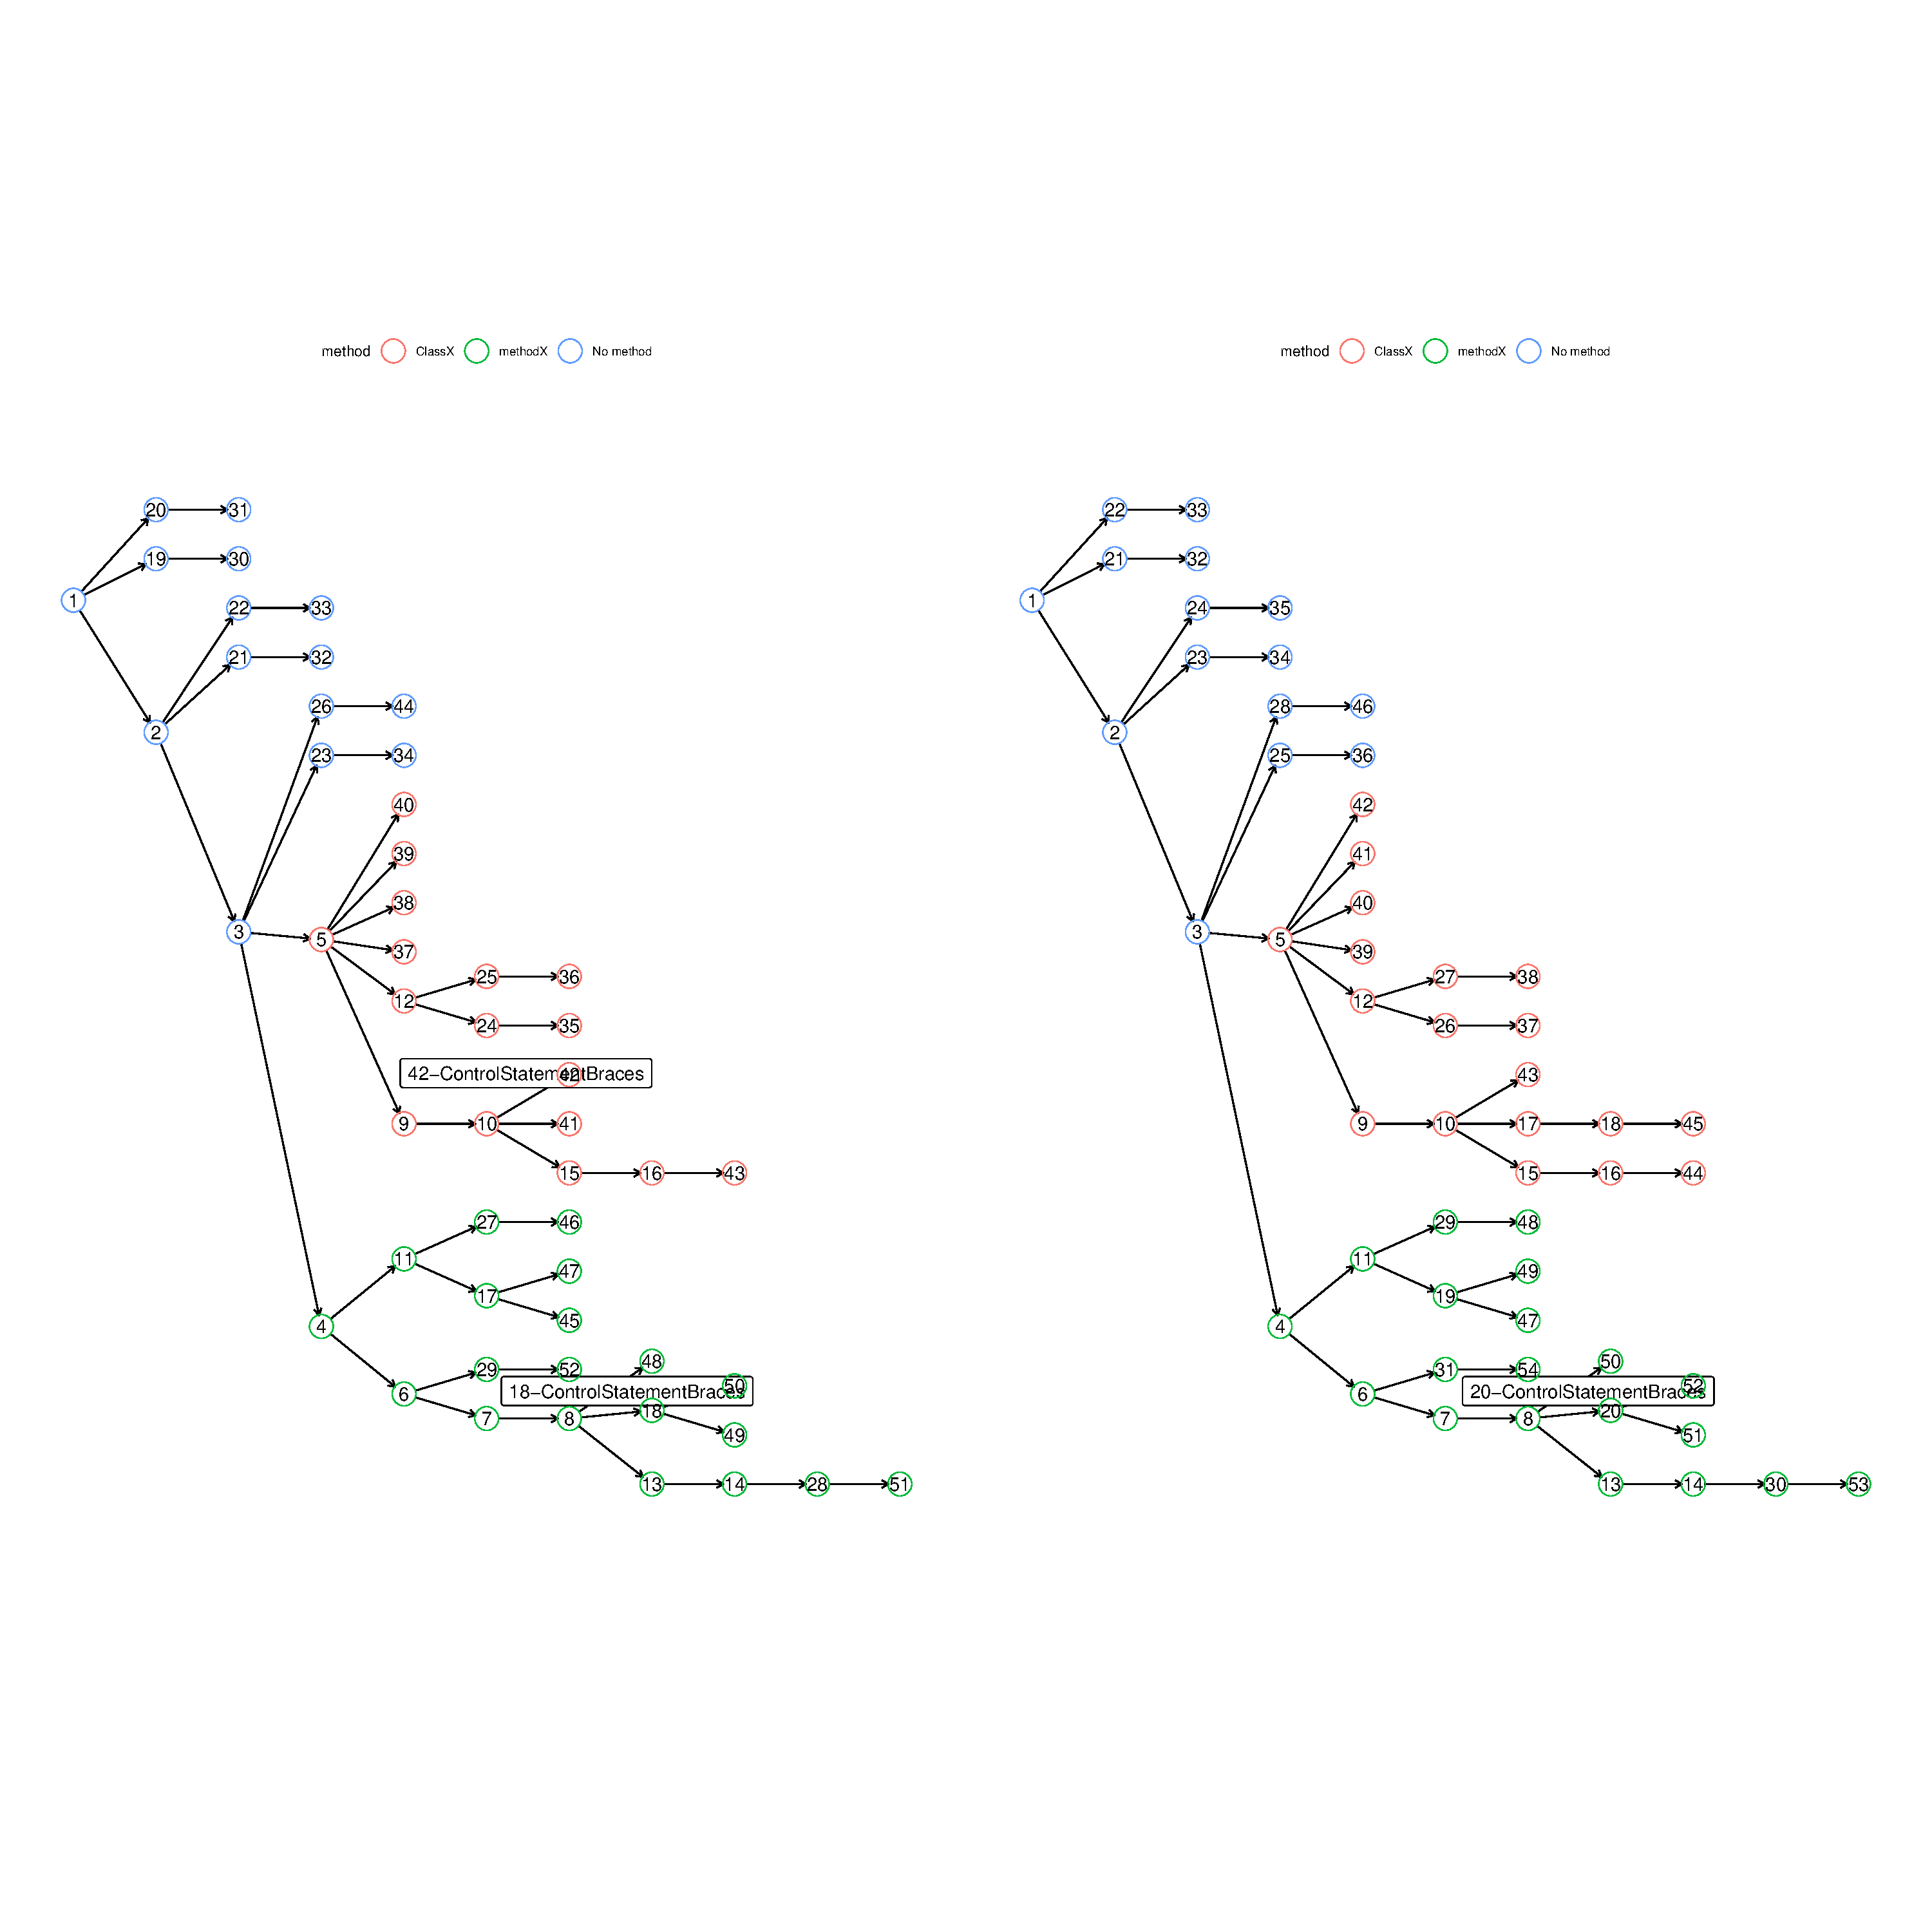
\includegraphics[width=1\linewidth]{match_algorithm_description_files/figure-latex/unnamed-chunk-4-1} \caption{Abstract Syntax Trees. New and old versions, with alerts \label{AST_compare_id_alerts}}\label{fig:unnamed-chunk-4}
\end{figure}

\normalsize

\small

\begin{figure}[H]
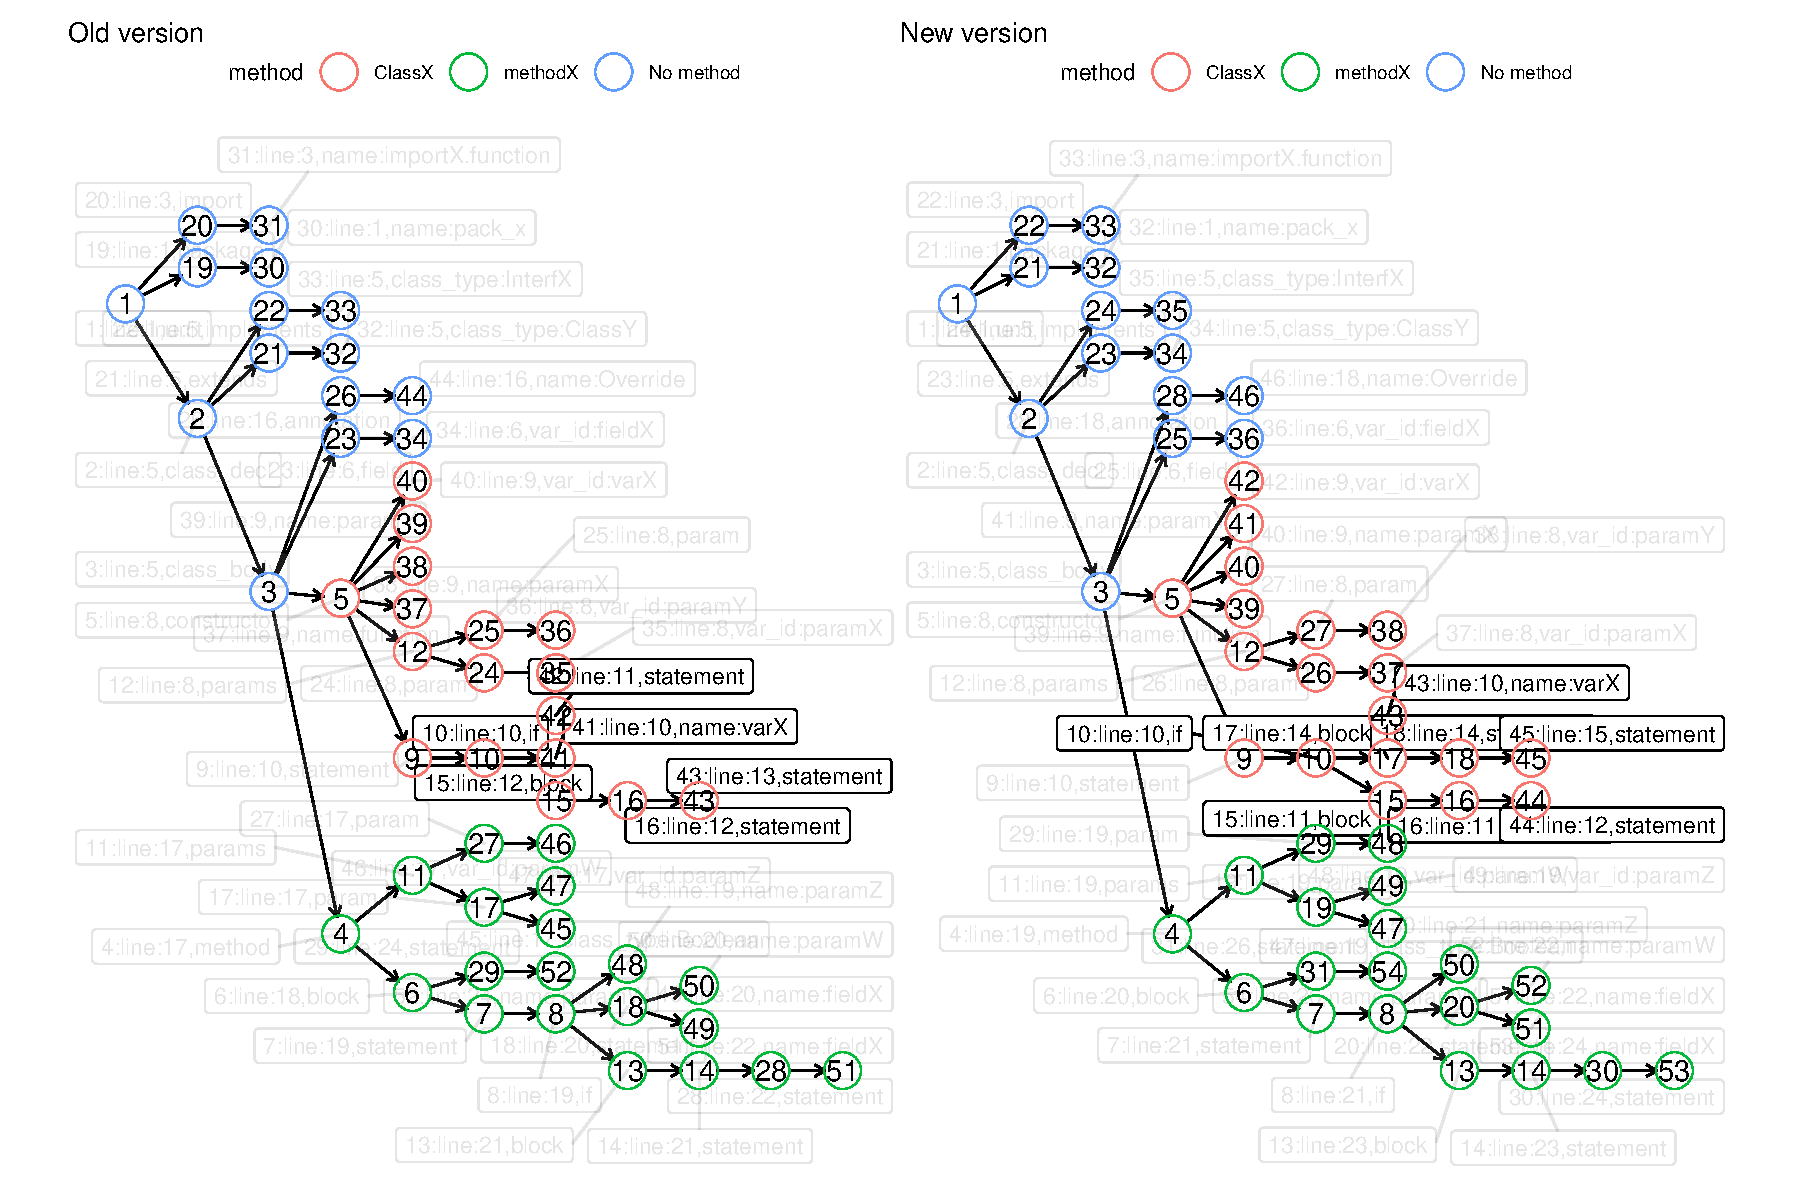
\includegraphics[width=1\linewidth]{match_algorithm_description_files/figure-latex/unnamed-chunk-5-1} \caption{Abstract Syntax Trees compared. New and old versions, with the type of some AST nodes \label{AST_compare}}\label{fig:unnamed-chunk-5}
\end{figure}

\normalsize

\textcolor{red}{Prof. Márcio, a diferença entre as árvores \ref{AST_compare_id_alerts} e \ref{AST_compare}, que coloquei na legenda agora, é que uma mostra os alertas e a outra mostra os tipos de nós da AST localizados perto do alerta que ficou nas duas versões. Se colocasse tudo junto ia embolar }

In Figure \ref{AST_with_alerts} the numbers inside the nodes are the
number of the group: nodes with the same number are equivalent. We
define that a node from an AST is equivalent to a node of the AST of the
subsequent version if:

\begin{itemize}
\item
  Considering the relation between the lines of the two versions
  constructed as we saw in Section \ref{map}, the nodes in both trees
  begin and end in related lines.
\item
  The nodes are of the same kind
\end{itemize}

\textcolor{red}{Prof. Márcio, sim, agora ser o mesmo nó significa apenas estar nas mesmas linhas (levando em conta o diff) e ser do mesmo tipo. As outras carascterísticas vão ser indicadas nas features que serão construídas mais pra frente}

\textcolor{red}{Prof. Márcio, eu fui colocando várias árvores pra tentar fazer as coisas passo a passo. Apresentei primeiro os nós equivalentes e depois coloquei os alertas. Mas agora eu apresentei só uma dessas duas árvores, com uma legenda melhor }

\small

\begin{figure}[H]
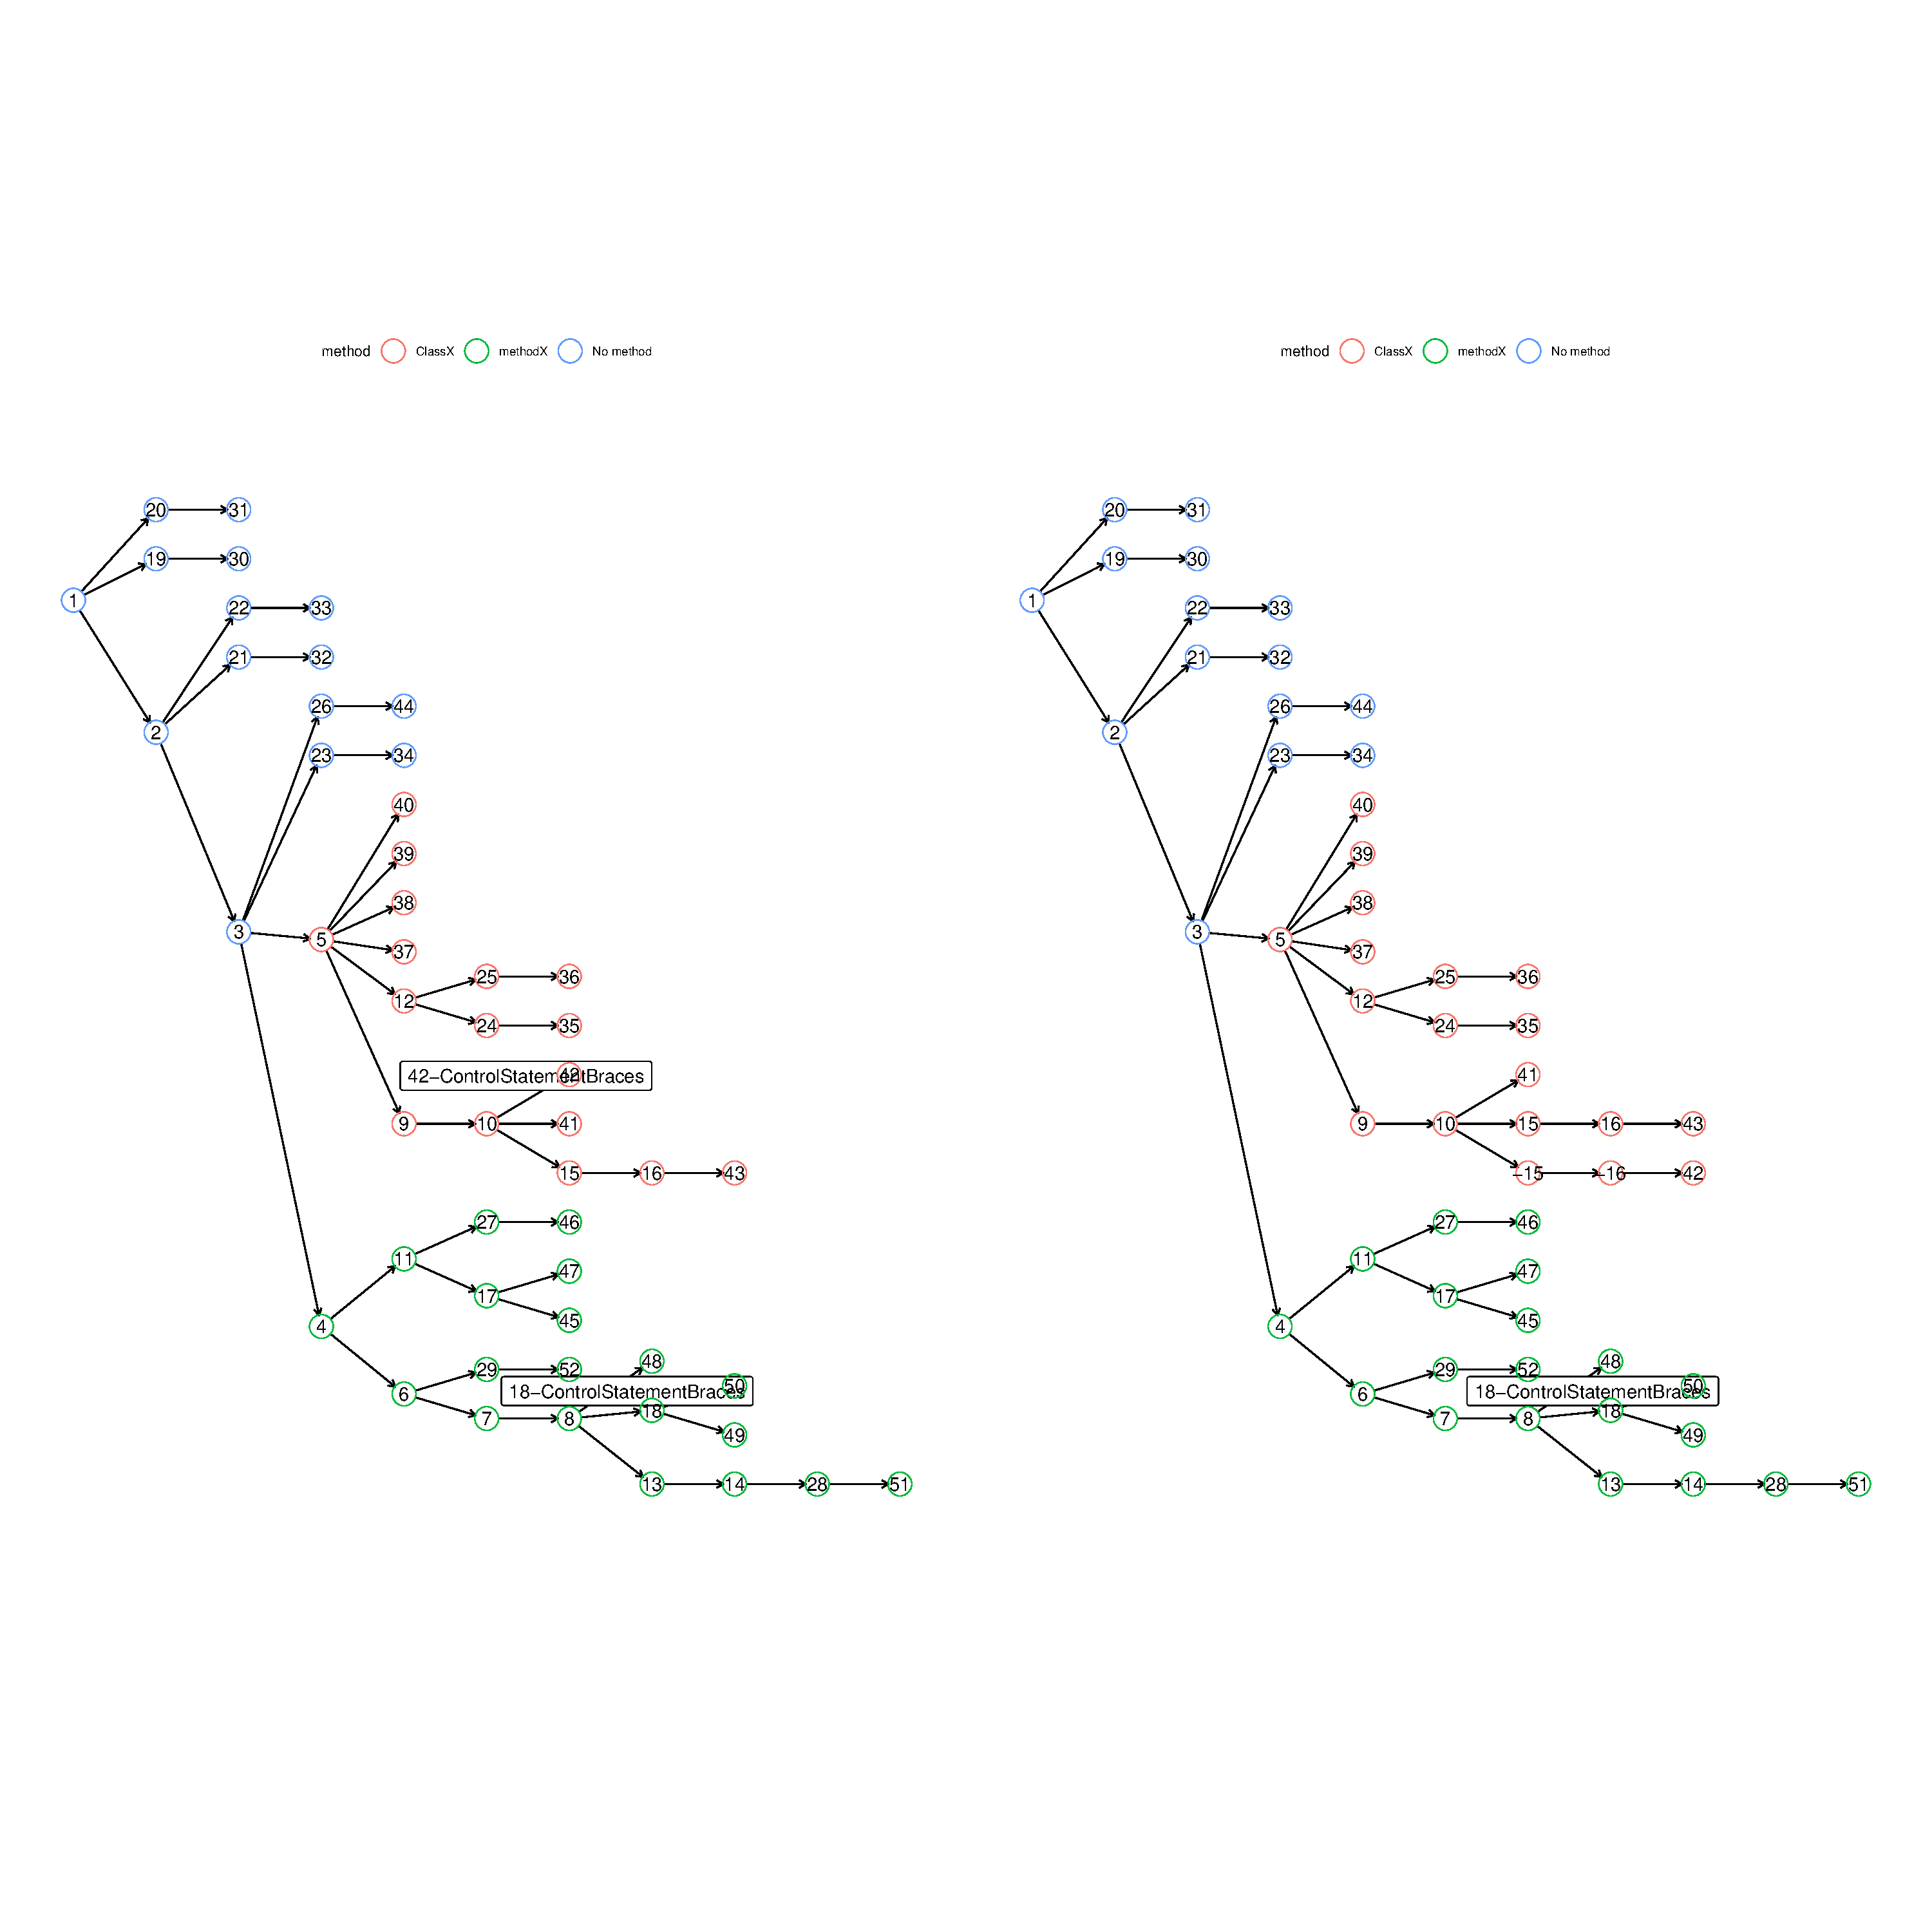
\includegraphics[width=1\linewidth]{match_algorithm_description_files/figure-latex/unnamed-chunk-6-1} \caption{Abstract Syntax Tree. Nodes with the same number are equivalent \label{AST_with_alerts}}\label{fig:unnamed-chunk-6}
\end{figure}

\normalsize

The path between the alert and the root of the AST can be seen in
\ref{AST_alert_1}

\small

\begin{figure}[H]
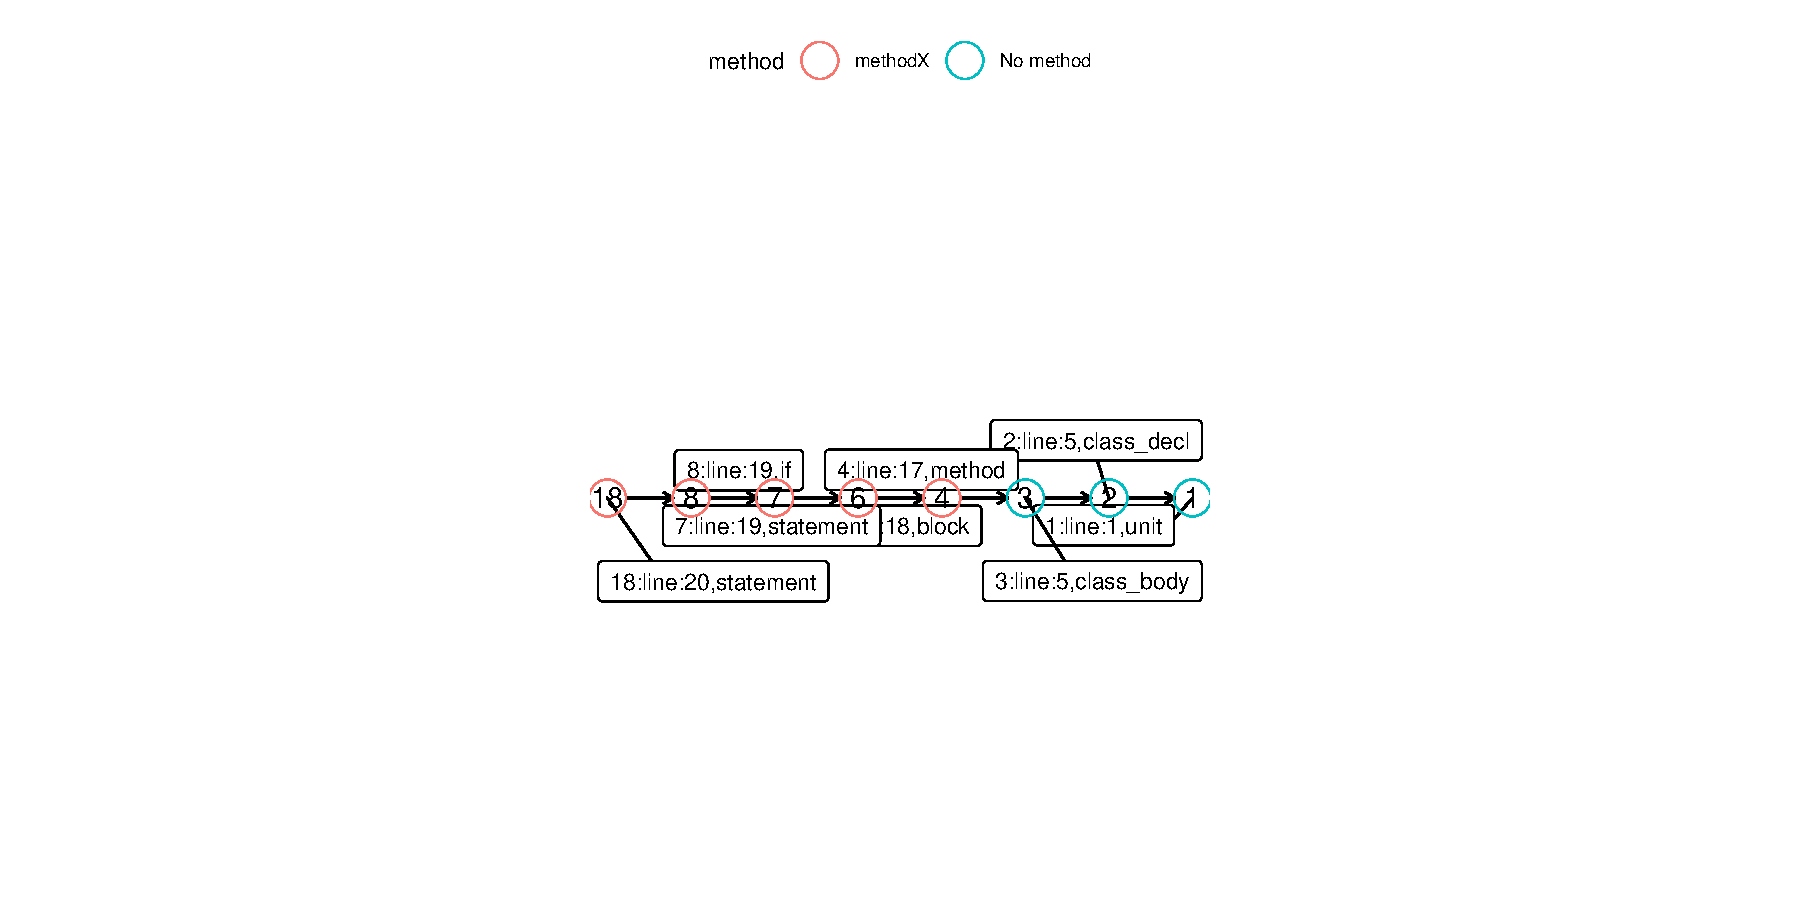
\includegraphics[width=1\linewidth]{match_algorithm_description_files/figure-latex/unnamed-chunk-7-1} \caption{Abstract Syntax Tree \label{AST_alert_1}}\label{fig:unnamed-chunk-7}
\end{figure}

\normalsize

The algorithm generates a set of features for each pair of alerts
\((n,o)\) with one element \(n\) coming from the old version and one
element \(o\) coming from the new version. The features do not lead to a
direct conclusion. It´s necessary to create a heuristic or statistical
learning algorithm that will decide the final verdict based on the
features.

We propose the following list of features:

\begin{itemize}
\item
  Same Rule: a boolean indicator that tells if the alerts are of the
  same type
\item
  Same Group ID: a boolean indicator that tells if the alerts are
  equivalent as defined in Figure \ref{AST_groups}
\item
  Same Method Group ID: a boolean indicator that tells if the alerts
  belong to the same method. We know the alert's method following the
  path from the alert´s node to the root. The first node of the kind
  ``method'' found in this path defines the alert's method. If this is
  the same for \(o\) and for \(n\), then they belong to the same method.
\item
  Same Method Name: a boolean indicator that tells if the alerts were
  found in a method with the same name.
\item
  Same Block: a boolean indicator that shows if the \(o\) and \(n\)
  belong to the same block. It is defined the same way the ``Same
  method'' indicator is defined.
\item
  Same Code: a boolean indicator that shows the nodes that generate the
  alert have the same programming code.
\item
  Same Method Code: a boolean indicator that shows that the methods that
  contain the nodes that generate the alert have the same programming
  code.
\item
  Line distance: \(o\) and \(n\) have a begin line \(b(o)\) and \(b(n)\)
  and an end line \(e(n)\) and \(e(n)\). Line distance is
  \(abs(mean(b(o), e(o)) - mean(b(n), e(n)))\)
\item
  Normalized line distance (block size): this is the line distance but
  normalized by the size of the last common node.
\item
  Normalized line distance (method size): this is the line distance but
  normalized by the size of the last common method (if there is no
  common method, it´s normalized by the side of the compilation unit).
\item
  Normalized line distance (compilation unit size): this is the line
  distance but normalized by the size of the compilation unit.
\end{itemize}

Table \ref{table_features} shows the combinations \((n,o)\) in the
example. There are \(2 \cdot 1 = 2\) combinations whereas we have two
alerts in the old version and one alert in the new one.

\small

\begin{table}[!h]

\caption{\label{tab:unnamed-chunk-8}Resulting features\label{table_features} }
\centering
\begin{tabular}[t]{l|l|l}
\hline
Alert combination & Feature & Value\\
\hline
\rowcolor{gray!6}   & Same Rule & TRUE\\

 & Same Group ID & TRUE\\

\rowcolor{gray!6}   & Same Method Group ID & TRUE\\

 & Same Method Name & TRUE\\

\rowcolor{gray!6}   & Same Block & TRUE\\

 & Same Code & TRUE\\

\rowcolor{gray!6}   & Same Method Code & TRUE\\

 & Line Distance & 0.00\\

\rowcolor{gray!6}   & Line Distance Normalized by Block Size & 0.00\\

 & Line Distance Normalized by Method Size & 0.00\\

\multirow[t]{-11}{*}{\raggedright\arraybackslash Line (Old version):20, Line (New version):22} & Line Distance Normalized by Compilation Unit Size & 0.00\\
\cline{1-3}
 & Same Rule & TRUE\\

\rowcolor{gray!6}   & Same Group ID & FALSE\\

 & Same Method Group ID & FALSE\\

\rowcolor{gray!6}   & Same Method Name & FALSE\\

 & Same Block & FALSE\\

\rowcolor{gray!6}   & Same Code & FALSE\\

 & Same Method Code & FALSE\\

\rowcolor{gray!6}   & Line Distance & 10.00\\

 & Line Distance Normalized by Block Size & 0.43\\

\rowcolor{gray!6}   & Line Distance Normalized by Method Size & 0.37\\

\multirow[t]{-11}{*}{\raggedright\arraybackslash Line (Old version):11, Line (New version):22} & Line Distance Normalized by Compilation Unit Size & 0.37\\
\hline
\end{tabular}
\end{table}

\normalsize

\small

\begin{verbatim}
## [1] "file"
## old_new.diff
\end{verbatim}

\normalsize

\newpage

\begin{landscape}

\subsubsection{Example: Renaming method} \label{example_rename_method}

In this example, the new and old versions have only one alert. The
method in which the alert happens is renamed from MethodX to methodZ.

\scriptsize

\begin{Shaded}
\begin{Highlighting}[]
\CommentTok{/*  1-                 */}\KeywordTok{package}\ImportTok{ pack_x;                                                /*  1-                 */package pack_x;}                                                
\CommentTok{/*  2-                 */}                                                               \CommentTok{/*  2-                 */}                                                               
\CommentTok{/*  3-                 */}\KeywordTok{import}\ImportTok{ importX.function;                                       /*  3-                 */import importX.function;}                                       
\CommentTok{/*  4-                 */}                                                               \CommentTok{/*  4-                 */}                                                               
\CommentTok{/*  5-                 */}\KeywordTok{class}\NormalTok{ ClassX }\KeywordTok{extends}\NormalTok{ ClassY }\KeywordTok{implements}\NormalTok{ InterfX \{               }\CommentTok{/*  5-                 */}\KeywordTok{class}\NormalTok{ ClassX }\KeywordTok{extends}\NormalTok{ ClassY }\KeywordTok{implements}\NormalTok{ InterfX \{               }
\CommentTok{/*  6-                 */}    \KeywordTok{private} \DataTypeTok{long}\NormalTok{ fieldX;                                       }\CommentTok{/*  6-                 */}    \KeywordTok{private} \DataTypeTok{long}\NormalTok{ fieldX;                                       }
\CommentTok{/*  7-                 */}                                                               \CommentTok{/*  7-                 */}                                                               
\CommentTok{/*  8-                 */}    \FunctionTok{ClassX}\NormalTok{(}\DataTypeTok{int}\NormalTok{ paramX, }\DataTypeTok{double}\NormalTok{ paramY) \{                                }\CommentTok{/*  8-                 */}    \FunctionTok{ClassX}\NormalTok{(}\DataTypeTok{int}\NormalTok{ paramX, }\DataTypeTok{double}\NormalTok{ paramY) \{                                }
\CommentTok{/*  9-                 */}        \DataTypeTok{int}\NormalTok{ varX = }\FunctionTok{function}\NormalTok{(paramX, paramY);                          }\CommentTok{/*  9-                 */}        \DataTypeTok{int}\NormalTok{ varX = }\FunctionTok{function}\NormalTok{(paramX, paramY);                           }
\CommentTok{/*   -                 *//*XXXXXXXXXXXXXXXXXXXXXXXXXXXXXXXXXXXXXX*/}                     \CommentTok{/* 10-                 */}        \KeywordTok{if}\NormalTok{ (varX == }\DecValTok{0}\NormalTok{)                                         }
\CommentTok{/* 10-                 */}        \KeywordTok{if}\NormalTok{ (varX == }\DecValTok{0}\NormalTok{)\{                                        }\CommentTok{/*   -                 *//*XXXXXXXXXXXXXXXXXXXXXXXXXXXXXXXXXXXXXX*/}                     
\CommentTok{/*   -                 *//*XXXXXXXXXXXXXXXXXXXXXXXXXXXXXXXXXXXXXX*/}                     \CommentTok{/* 11-                 */}\NormalTok{        \{                                                      }
\CommentTok{/* 11-                 */}            \KeywordTok{this}\NormalTok{.}\FunctionTok{fieldX}\NormalTok{ = }\DecValTok{1}\NormalTok{;                                   }\CommentTok{/* 12-                 */}            \KeywordTok{this}\NormalTok{.}\FunctionTok{fieldX}\NormalTok{ = }\DecValTok{1}\NormalTok{;                                   }
\CommentTok{/* 12-                 */}\NormalTok{        \}                                                      }\CommentTok{/*   -                 *//*XXXXXXXXXXXXXXXXXXXXXXXXXXXXXXXXXXXXXX*/}                     
\CommentTok{/*   -                 *//*XXXXXXXXXXXXXXXXXXXXXXXXXXXXXXXXXXXXXX*/}                     \CommentTok{/* 13-                 */}\NormalTok{        \}                                                                }
\CommentTok{/* 13-                 */}        \KeywordTok{else}\NormalTok{\{                                                  }\CommentTok{/* 14-                 */}        \KeywordTok{else}\NormalTok{\{                                                  }
\CommentTok{/* 14-                 */}            \KeywordTok{this}\NormalTok{.}\FunctionTok{fieldX}\NormalTok{ = }\DecValTok{0}\NormalTok{;                                   }\CommentTok{/* 15-                 */}            \KeywordTok{this}\NormalTok{.}\FunctionTok{fieldX}\NormalTok{ = }\DecValTok{0}\NormalTok{;                                   }
\CommentTok{/* 15-                 */}\NormalTok{        \}                                                      }\CommentTok{/* 16-                 */}\NormalTok{        \}                                                      }
\CommentTok{/* 16-                 */}\NormalTok{    \}                                                          }\CommentTok{/* 17-                 */}\NormalTok{    \}                                                          }
\CommentTok{/* 17-                 */}    \AttributeTok{@Override}                                                  \CommentTok{/* 18-                 */}    \AttributeTok{@Override}                                                  
\CommentTok{/* 18-                 */}    \KeywordTok{public} \DataTypeTok{int} \FunctionTok{methodX}\NormalTok{(}\DataTypeTok{int}\NormalTok{ paramW, }\BuiltInTok{Boolean}\NormalTok{ paramZ)             }\CommentTok{/*   -                 *//*XXXXXXXXXXXXXXXXXXXXXXXXXXXXXXXXXXXXXX*/}                     
\CommentTok{/*   -                 *//*XXXXXXXXXXXXXXXXXXXXXXXXXXXXXXXXXXXXXX*/}                     \CommentTok{/* 19-                 */}    \KeywordTok{public} \DataTypeTok{int} \FunctionTok{methodZ}\NormalTok{(}\DataTypeTok{int}\NormalTok{ paramW, }\BuiltInTok{Boolean}\NormalTok{ paramZ)             }
\CommentTok{/* 19-                 */}\NormalTok{    \{                                                          }\CommentTok{/* 20-                 */}\NormalTok{    \{                                                          }
\CommentTok{/* 20-                 */}        \KeywordTok{if}\NormalTok{ (paramZ)                                            }\CommentTok{/* 21-                 */}        \KeywordTok{if}\NormalTok{ (paramZ)                                            }
\CommentTok{/* 21-ControlStateme   */}\NormalTok{            fieldX = paramW;                                   }\CommentTok{/* 22-ControlStateme   */}\NormalTok{            fieldX = paramW;                                   }
\CommentTok{/* 22-                 */}        \KeywordTok{else}\NormalTok{\{                                                  }\CommentTok{/* 23-                 */}        \KeywordTok{else}\NormalTok{\{                                                  }
\CommentTok{/* 23-                 */}\NormalTok{            fieldX = }\DecValTok{0}\NormalTok{;                                        }\CommentTok{/* 24-                 */}\NormalTok{            fieldX = }\DecValTok{0}\NormalTok{;                                        }
\CommentTok{/* 24-                 */}\NormalTok{        \}                                                      }\CommentTok{/* 25-                 */}\NormalTok{        \}                                                      }
\CommentTok{/* 25-                 */}        \KeywordTok{return}\NormalTok{ paramW + }\KeywordTok{this}\NormalTok{.}\FunctionTok{fieldX}\NormalTok{;                           }\CommentTok{/* 26-                 */}        \KeywordTok{return}\NormalTok{ paramW + }\KeywordTok{this}\NormalTok{.}\FunctionTok{fieldX}\NormalTok{;                           }
\CommentTok{/* 26-                 */}\NormalTok{     \}                                                         }\CommentTok{/* 27-                 */}\NormalTok{     \}                                                         }
\CommentTok{/* 27-                 */}\NormalTok{\}                                                              }\CommentTok{/* 28-                 */}\NormalTok{\}                                                              }
\end{Highlighting}
\end{Shaded}

\normalsize

\begin{figure}
\centering

\includegraphics{figures/fake.png}
\caption{Comparison between old and new version
\label{comparison_rename}}
\end{figure}

\end{landscape}

\newpage

In the Table \ref{features_rename} we can see that the features ``Same
Method Name'' and ``Same Method Group ID'' are now FALSE.

\small

\begin{table}[!h]

\caption{\label{tab:unnamed-chunk-10}Resulting features: rename method example \label{features_rename} }
\centering
\begin{tabular}[t]{l|l|l}
\hline
Alert combination & Feature & Value\\
\hline
\rowcolor{gray!6}   & Same Rule & TRUE\\

 & Same Group ID & TRUE\\

\rowcolor{gray!6}   & Same Method Group ID & FALSE\\

 & Same Method Name & FALSE\\

\rowcolor{gray!6}   & Same Block & TRUE\\

 & Same Code & TRUE\\

\rowcolor{gray!6}   & Same Method Code & FALSE\\

 & Line Distance & 0.00\\

\rowcolor{gray!6}   & Line Distance Normalized by Block Size & 0.00\\

 & Line Distance Normalized by Method Size & 0.00\\

\multirow[t]{-11}{*}{\raggedright\arraybackslash Line (Old version):21, Line (New version):22} & Line Distance Normalized by Compilation Unit Size & 0.00\\
\hline
\end{tabular}
\end{table}

\normalsize

\newpage

\begin{landscape}

\subsubsection{Example: including a statement before} \label{example_including_statement}

\small

\begin{verbatim}
## [1] "file"
## old_new.diff
\end{verbatim}

\normalsize

In this example, a new statement is included before the alert.

\scriptsize

\begin{Shaded}
\begin{Highlighting}[]
\CommentTok{/*  1-                 */}\KeywordTok{package}\ImportTok{ pack_x;                                                /*  1-                 */package pack_x;}                                                
\CommentTok{/*  2-                 */}                                                               \CommentTok{/*  2-                 */}                                                               
\CommentTok{/*  3-                 */}\KeywordTok{import}\ImportTok{ importX.function;                                       /*  3-                 */import importX.function;}                                       
\CommentTok{/*  4-                 */}                                                               \CommentTok{/*  4-                 */}                                                               
\CommentTok{/*  5-                 */}\KeywordTok{class}\NormalTok{ ClassX }\KeywordTok{extends}\NormalTok{ ClassY }\KeywordTok{implements}\NormalTok{ InterfX \{               }\CommentTok{/*  5-                 */}\KeywordTok{class}\NormalTok{ ClassX }\KeywordTok{extends}\NormalTok{ ClassY }\KeywordTok{implements}\NormalTok{ InterfX \{               }
\CommentTok{/*  6-                 */}    \KeywordTok{private} \DataTypeTok{long}\NormalTok{ fieldX;                                       }\CommentTok{/*  6-                 */}    \KeywordTok{private} \DataTypeTok{long}\NormalTok{ fieldX;                                       }
\CommentTok{/*  7-                 */}                                                               \CommentTok{/*  7-                 */}                                                               
\CommentTok{/*  8-                 */}    \FunctionTok{ClassX}\NormalTok{(}\DataTypeTok{int}\NormalTok{ paramX, }\DataTypeTok{double}\NormalTok{ paramY) \{                                }\CommentTok{/*  8-                 */}    \FunctionTok{ClassX}\NormalTok{(}\DataTypeTok{int}\NormalTok{ paramX, }\DataTypeTok{double}\NormalTok{ paramY) \{                                }
\CommentTok{/*  9-                 */}        \DataTypeTok{int}\NormalTok{ varX = }\FunctionTok{function}\NormalTok{(paramX, paramY);                          }\CommentTok{/*  9-                 */}        \DataTypeTok{int}\NormalTok{ varX = }\FunctionTok{function}\NormalTok{(paramX, paramY);                           }
\CommentTok{/* 10-                 */}        \KeywordTok{if}\NormalTok{ (varX == }\DecValTok{0}\NormalTok{)                                         }\CommentTok{/* 10-                 */}        \KeywordTok{if}\NormalTok{ (varX == }\DecValTok{0}\NormalTok{)                                         }
\CommentTok{/* 11-                 */}\NormalTok{        \{                                                      }\CommentTok{/* 11-                 */}\NormalTok{        \{                                                      }
\CommentTok{/* 12-                 */}            \KeywordTok{this}\NormalTok{.}\FunctionTok{fieldX}\NormalTok{ = }\DecValTok{1}\NormalTok{;                                   }\CommentTok{/* 12-                 */}            \KeywordTok{this}\NormalTok{.}\FunctionTok{fieldX}\NormalTok{ = }\DecValTok{1}\NormalTok{;                                   }
\CommentTok{/* 13-                 */}\NormalTok{        \}                                                                }\CommentTok{/* 13-                 */}\NormalTok{        \}                                                                  }
\CommentTok{/* 14-                 */}        \KeywordTok{else}\NormalTok{\{                                                  }\CommentTok{/* 14-                 */}        \KeywordTok{else}\NormalTok{\{                                                  }
\CommentTok{/* 15-                 */}            \KeywordTok{this}\NormalTok{.}\FunctionTok{fieldX}\NormalTok{ = }\DecValTok{0}\NormalTok{;                                   }\CommentTok{/* 15-                 */}            \KeywordTok{this}\NormalTok{.}\FunctionTok{fieldX}\NormalTok{ = }\DecValTok{0}\NormalTok{;                                   }
\CommentTok{/* 16-                 */}\NormalTok{        \}                                                      }\CommentTok{/* 16-                 */}\NormalTok{        \}                                                      }
\CommentTok{/* 17-                 */}\NormalTok{    \}                                                          }\CommentTok{/* 17-                 */}\NormalTok{    \}                                                          }
\CommentTok{/* 18-                 */}    \AttributeTok{@Override}                                                  \CommentTok{/* 18-                 */}    \AttributeTok{@Override}                                                  
\CommentTok{/* 19-                 */}    \KeywordTok{public} \DataTypeTok{int} \FunctionTok{methodZ}\NormalTok{(}\DataTypeTok{int}\NormalTok{ paramW, }\BuiltInTok{Boolean}\NormalTok{ paramZ)             }\CommentTok{/* 19-                 */}    \KeywordTok{public} \DataTypeTok{int} \FunctionTok{methodZ}\NormalTok{(}\DataTypeTok{int}\NormalTok{ paramW, }\BuiltInTok{Boolean}\NormalTok{ paramZ)             }
\CommentTok{/* 20-                 */}\NormalTok{    \{                                                          }\CommentTok{/* 20-                 */}\NormalTok{    \{                                                          }
\CommentTok{/*   -                 *//*XXXXXXXXXXXXXXXXXXXXXXXXXXXXXXXXXXXXXX*/}                     \CommentTok{/* 21-                 */}\NormalTok{       paramT = }\DecValTok{0}\NormalTok{;                                                    }
\CommentTok{/* 21-                 */}        \KeywordTok{if}\NormalTok{ (paramZ)                                            }\CommentTok{/* 22-                 */}        \KeywordTok{if}\NormalTok{ (paramZ)                                            }
\CommentTok{/* 22-ControlStateme   */}\NormalTok{            fieldX = paramW;                                   }\CommentTok{/* 23-ControlStateme   */}\NormalTok{            fieldX = paramW;                                   }
\CommentTok{/* 23-                 */}        \KeywordTok{else}\NormalTok{\{                                                  }\CommentTok{/* 24-                 */}        \KeywordTok{else}\NormalTok{\{                                                  }
\CommentTok{/* 24-                 */}\NormalTok{            fieldX = }\DecValTok{0}\NormalTok{;                                        }\CommentTok{/* 25-                 */}\NormalTok{            fieldX = }\DecValTok{0}\NormalTok{;                                        }
\CommentTok{/* 25-                 */}\NormalTok{        \}                                                      }\CommentTok{/* 26-                 */}\NormalTok{        \}                                                      }
\CommentTok{/* 26-                 */}        \KeywordTok{return}\NormalTok{ paramW + }\KeywordTok{this}\NormalTok{.}\FunctionTok{fieldX}\NormalTok{;                           }\CommentTok{/* 27-                 */}        \KeywordTok{return}\NormalTok{ paramW + }\KeywordTok{this}\NormalTok{.}\FunctionTok{fieldX}\NormalTok{;                           }
\CommentTok{/* 27-                 */}\NormalTok{     \}                                                         }\CommentTok{/* 28-                 */}\NormalTok{     \}                                                         }
\CommentTok{/* 28-                 */}\NormalTok{\}                                                              }\CommentTok{/* 29-                 */}\NormalTok{\}                                                              }
\end{Highlighting}
\end{Shaded}

\normalsize

\begin{figure}
\centering

\includegraphics{figures/fake.png}
\caption{Comparison between old and new version
\label{comparison_include_statement_before}}
\end{figure}

\end{landscape}

\newpage

In the Table \ref{include_statement_before} we can see that the features
are not affected by this new statement.

\small

\begin{table}[!h]

\caption{\label{tab:unnamed-chunk-12}Resulting features: statement included before \label{include_statement_before} }
\centering
\begin{tabular}[t]{l|l|l}
\hline
Alert combination & Feature & Value\\
\hline
\rowcolor{gray!6}   & Same Rule & TRUE\\

 & Same Group ID & TRUE\\

\rowcolor{gray!6}   & Same Method Group ID & TRUE\\

 & Same Method Name & TRUE\\

\rowcolor{gray!6}   & Same Block & TRUE\\

 & Same Code & TRUE\\

\rowcolor{gray!6}   & Same Method Code & FALSE\\

 & Line Distance & 0.00\\

\rowcolor{gray!6}   & Line Distance Normalized by Block Size & 0.00\\

 & Line Distance Normalized by Method Size & 0.00\\

\multirow[t]{-11}{*}{\raggedright\arraybackslash Line (Old version):22, Line (New version):23} & Line Distance Normalized by Compilation Unit Size & 0.00\\
\hline
\end{tabular}
\end{table}

\normalsize

\newpage

\begin{landscape}

\subsubsection{Example: nesting the alert in an if statement} \label{example_nested_in_other_if}

\small

\begin{verbatim}
## [1] "file"
## old_new.diff
\end{verbatim}

\normalsize

\scriptsize

\begin{Shaded}
\begin{Highlighting}[]
\CommentTok{/*  1-                 */}\KeywordTok{package}\ImportTok{ pack_x;                                                /*  1-                 */package pack_x;}                                                
\CommentTok{/*  2-                 */}                                                               \CommentTok{/*  2-                 */}                                                               
\CommentTok{/*  3-                 */}\KeywordTok{import}\ImportTok{ importX.function;                                       /*  3-                 */import importX.function;}                                       
\CommentTok{/*  4-                 */}                                                               \CommentTok{/*  4-                 */}                                                               
\CommentTok{/*  5-                 */}\KeywordTok{class}\NormalTok{ ClassX }\KeywordTok{extends}\NormalTok{ ClassY }\KeywordTok{implements}\NormalTok{ InterfX \{               }\CommentTok{/*  5-                 */}\KeywordTok{class}\NormalTok{ ClassX }\KeywordTok{extends}\NormalTok{ ClassY }\KeywordTok{implements}\NormalTok{ InterfX \{               }
\CommentTok{/*  6-                 */}    \KeywordTok{private} \DataTypeTok{long}\NormalTok{ fieldX;                                       }\CommentTok{/*  6-                 */}    \KeywordTok{private} \DataTypeTok{long}\NormalTok{ fieldX;                                       }
\CommentTok{/*  7-                 */}                                                               \CommentTok{/*  7-                 */}                                                               
\CommentTok{/*  8-                 */}    \FunctionTok{ClassX}\NormalTok{(}\DataTypeTok{int}\NormalTok{ paramX, }\DataTypeTok{double}\NormalTok{ paramY) \{                                }\CommentTok{/*  8-                 */}    \FunctionTok{ClassX}\NormalTok{(}\DataTypeTok{int}\NormalTok{ paramX, }\DataTypeTok{double}\NormalTok{ paramY) \{                                }
\CommentTok{/*  9-                 */}        \DataTypeTok{int}\NormalTok{ varX = }\FunctionTok{function}\NormalTok{(paramX, paramY);                          }\CommentTok{/*  9-                 */}        \DataTypeTok{int}\NormalTok{ varX = }\FunctionTok{function}\NormalTok{(paramX, paramY);                           }
\CommentTok{/* 10-                 */}        \KeywordTok{if}\NormalTok{ (varX == }\DecValTok{0}\NormalTok{)                                         }\CommentTok{/* 10-                 */}        \KeywordTok{if}\NormalTok{ (varX == }\DecValTok{0}\NormalTok{)                                         }
\CommentTok{/* 11-                 */}\NormalTok{        \{                                                      }\CommentTok{/* 11-                 */}\NormalTok{        \{                                                      }
\CommentTok{/* 12-                 */}            \KeywordTok{this}\NormalTok{.}\FunctionTok{fieldX}\NormalTok{ = }\DecValTok{1}\NormalTok{;                                   }\CommentTok{/* 12-                 */}            \KeywordTok{this}\NormalTok{.}\FunctionTok{fieldX}\NormalTok{ = }\DecValTok{1}\NormalTok{;                                   }
\CommentTok{/* 13-                 */}\NormalTok{        \}                                                                }\CommentTok{/* 13-                 */}\NormalTok{        \}                                                                  }
\CommentTok{/* 14-                 */}        \KeywordTok{else}\NormalTok{\{                                                  }\CommentTok{/* 14-                 */}        \KeywordTok{else}\NormalTok{\{                                                  }
\CommentTok{/* 15-                 */}            \KeywordTok{this}\NormalTok{.}\FunctionTok{fieldX}\NormalTok{ = }\DecValTok{0}\NormalTok{;                                   }\CommentTok{/* 15-                 */}            \KeywordTok{this}\NormalTok{.}\FunctionTok{fieldX}\NormalTok{ = }\DecValTok{0}\NormalTok{;                                   }
\CommentTok{/* 16-                 */}\NormalTok{        \}                                                      }\CommentTok{/* 16-                 */}\NormalTok{        \}                                                      }
\CommentTok{/* 17-                 */}\NormalTok{    \}                                                          }\CommentTok{/* 17-                 */}\NormalTok{    \}                                                          }
\CommentTok{/* 18-                 */}    \AttributeTok{@Override}                                                  \CommentTok{/* 18-                 */}    \AttributeTok{@Override}                                                  
\CommentTok{/* 19-                 */}    \KeywordTok{public} \DataTypeTok{int} \FunctionTok{methodZ}\NormalTok{(}\DataTypeTok{int}\NormalTok{ paramW, }\BuiltInTok{Boolean}\NormalTok{ paramZ)             }\CommentTok{/* 19-                 */}    \KeywordTok{public} \DataTypeTok{int} \FunctionTok{methodZ}\NormalTok{(}\DataTypeTok{int}\NormalTok{ paramW, }\BuiltInTok{Boolean}\NormalTok{ paramZ)             }
\CommentTok{/* 20-                 */}\NormalTok{    \{                                                          }\CommentTok{/* 20-                 */}\NormalTok{    \{                                                          }
\CommentTok{/*   -                 *//*XXXXXXXXXXXXXXXXXXXXXXXXXXXXXXXXXXXXXX*/}                     \CommentTok{/* 21-                 */}       \KeywordTok{if}\NormalTok{(paramZ == }\DecValTok{0}\NormalTok{)\{                                               }
\CommentTok{/* 21-                 */}        \KeywordTok{if}\NormalTok{ (paramZ)                                            }\CommentTok{/*   -                 *//*XXXXXXXXXXXXXXXXXXXXXXXXXXXXXXXXXXXXXX*/}                     
\CommentTok{/*   -                 *//*XXXXXXXXXXXXXXXXXXXXXXXXXXXXXXXXXXXXXX*/}                     \CommentTok{/* 22-                 */}            \KeywordTok{if}\NormalTok{ (paramZ)                                        }
\CommentTok{/* 22-ControlStateme   */}\NormalTok{            fieldX = paramW;                                   }\CommentTok{/*   -                 *//*XXXXXXXXXXXXXXXXXXXXXXXXXXXXXXXXXXXXXX*/}                     
\CommentTok{/*   -                 *//*XXXXXXXXXXXXXXXXXXXXXXXXXXXXXXXXXXXXXX*/}                     \CommentTok{/* 23-ControlStateme   */}\NormalTok{                fieldX = paramW;                               }
\CommentTok{/* 23-                 */}        \KeywordTok{else}\NormalTok{\{                                                  }\CommentTok{/*   -                 *//*XXXXXXXXXXXXXXXXXXXXXXXXXXXXXXXXXXXXXX*/}                     
\CommentTok{/*   -                 *//*XXXXXXXXXXXXXXXXXXXXXXXXXXXXXXXXXXXXXX*/}                     \CommentTok{/* 24-                 */}            \KeywordTok{else}\NormalTok{\{                                              }
\CommentTok{/* 24-                 */}\NormalTok{            fieldX = }\DecValTok{0}\NormalTok{;                                        }\CommentTok{/*   -                 *//*XXXXXXXXXXXXXXXXXXXXXXXXXXXXXXXXXXXXXX*/}                     
\CommentTok{/*   -                 *//*XXXXXXXXXXXXXXXXXXXXXXXXXXXXXXXXXXXXXX*/}                     \CommentTok{/* 25-                 */}\NormalTok{                fieldX = }\DecValTok{0}\NormalTok{;                                    }
\CommentTok{/* 25-                 */}\NormalTok{        \}                                                      }\CommentTok{/*   -                 *//*XXXXXXXXXXXXXXXXXXXXXXXXXXXXXXXXXXXXXX*/}                     
\CommentTok{/*   -                 *//*XXXXXXXXXXXXXXXXXXXXXXXXXXXXXXXXXXXXXX*/}                     \CommentTok{/* 26-                 */}\NormalTok{            \}                                                  }
\CommentTok{/*   -                 *//*XXXXXXXXXXXXXXXXXXXXXXXXXXXXXXXXXXXXXX*/}                     \CommentTok{/* 27-                 */}\NormalTok{       \}                                                                 }
\CommentTok{/*   -                 *//*XXXXXXXXXXXXXXXXXXXXXXXXXXXXXXXXXXXXXX*/}                     \CommentTok{/* 28-                 */}       \KeywordTok{else}\NormalTok{\{                                                      }
\CommentTok{/*   -                 *//*XXXXXXXXXXXXXXXXXXXXXXXXXXXXXXXXXXXXXX*/}                     \CommentTok{/* 29-                 */}\NormalTok{           fieldX = }\DecValTok{1}\NormalTok{;                                                }
\CommentTok{/*   -                 *//*XXXXXXXXXXXXXXXXXXXXXXXXXXXXXXXXXXXXXX*/}                     \CommentTok{/* 30-                 */}\NormalTok{       \}                                                              }
\CommentTok{/* 26-                 */}        \KeywordTok{return}\NormalTok{ paramW + }\KeywordTok{this}\NormalTok{.}\FunctionTok{fieldX}\NormalTok{;                           }\CommentTok{/* 31-                 */}        \KeywordTok{return}\NormalTok{ paramW + }\KeywordTok{this}\NormalTok{.}\FunctionTok{fieldX}\NormalTok{;                           }
\CommentTok{/* 27-                 */}\NormalTok{     \}                                                         }\CommentTok{/* 32-                 */}\NormalTok{     \}                                                         }
\CommentTok{/* 28-                 */}\NormalTok{\}                                                              }\CommentTok{/* 33-                 */}\NormalTok{\}                                                              }
\end{Highlighting}
\end{Shaded}

\normalsize

\begin{figure}
\centering

\includegraphics{figures/fake.png}
\caption{Comparison between old and new version
\label{comparison_nested_in_other_if}}
\end{figure}

\end{landscape}

\newpage

In the Table \ref{nested_in_other_if} we can see that the algorithm does
not recognize the two nodes as equivalent, but other features can lead
us to the conclusion that the alert is still open.

\small

\begin{table}[!h]

\caption{\label{tab:unnamed-chunk-14}Resulting features: statement included before \label{nested_in_other_if} }
\centering
\begin{tabular}[t]{l|l|l}
\hline
Alert combination & Feature & Value\\
\hline
\rowcolor{gray!6}   & Same Rule & TRUE\\

 & Same Group ID & FALSE\\

\rowcolor{gray!6}   & Same Method Group ID & TRUE\\

 & Same Method Name & TRUE\\

\rowcolor{gray!6}   & Same Block & FALSE\\

 & Same Code & TRUE\\

\rowcolor{gray!6}   & Same Method Code & FALSE\\

 & Line Distance & 1.00\\

\rowcolor{gray!6}   & Line Distance Normalized by Block Size & 0.06\\

 & Line Distance Normalized by Method Size & 0.06\\

\multirow[t]{-11}{*}{\raggedright\arraybackslash Line (Old version):22, Line (New version):23} & Line Distance Normalized by Compilation Unit Size & 0.03\\
\hline
\end{tabular}
\end{table}

\normalsize

\newpage

\begin{landscape}

\subsubsection{Example: editing the line that generates the alert} \label{example_editing_line}

\small

\begin{verbatim}
## [1] "file"
## old_new.diff
\end{verbatim}

\normalsize

\scriptsize

\begin{Shaded}
\begin{Highlighting}[]
\CommentTok{/*  1-                 */}\KeywordTok{package}\ImportTok{ pack_x;                                                /*  1-                 */package pack_x;}                                                
\CommentTok{/*  2-                 */}                                                               \CommentTok{/*  2-                 */}                                                               
\CommentTok{/*  3-                 */}\KeywordTok{import}\ImportTok{ importX.function;                                       /*  3-                 */import importX.function;}                                       
\CommentTok{/*  4-                 */}                                                               \CommentTok{/*  4-                 */}                                                               
\CommentTok{/*  5-                 */}\KeywordTok{class}\NormalTok{ ClassX }\KeywordTok{extends}\NormalTok{ ClassY }\KeywordTok{implements}\NormalTok{ InterfX \{               }\CommentTok{/*  5-                 */}\KeywordTok{class}\NormalTok{ ClassX }\KeywordTok{extends}\NormalTok{ ClassY }\KeywordTok{implements}\NormalTok{ InterfX \{               }
\CommentTok{/*  6-                 */}    \KeywordTok{private} \DataTypeTok{long}\NormalTok{ fieldX;                                       }\CommentTok{/*  6-                 */}    \KeywordTok{private} \DataTypeTok{long}\NormalTok{ fieldX;                                       }
\CommentTok{/*  7-                 */}                                                               \CommentTok{/*  7-                 */}                                                               
\CommentTok{/*  8-                 */}    \FunctionTok{ClassX}\NormalTok{(}\DataTypeTok{int}\NormalTok{ paramX, }\DataTypeTok{double}\NormalTok{ paramY) \{                                }\CommentTok{/*  8-                 */}    \FunctionTok{ClassX}\NormalTok{(}\DataTypeTok{int}\NormalTok{ paramX, }\DataTypeTok{double}\NormalTok{ paramY) \{                                }
\CommentTok{/*  9-                 */}        \DataTypeTok{int}\NormalTok{ varX = }\FunctionTok{function}\NormalTok{(paramX, paramY);                          }\CommentTok{/*  9-                 */}        \DataTypeTok{int}\NormalTok{ varX = }\FunctionTok{function}\NormalTok{(paramX, paramY);                           }
\CommentTok{/* 10-                 */}        \KeywordTok{if}\NormalTok{ (varX == }\DecValTok{0}\NormalTok{)                                         }\CommentTok{/* 10-                 */}        \KeywordTok{if}\NormalTok{ (varX == }\DecValTok{0}\NormalTok{)                                         }
\CommentTok{/* 11-                 */}\NormalTok{        \{                                                      }\CommentTok{/* 11-                 */}\NormalTok{        \{                                                      }
\CommentTok{/* 12-                 */}            \KeywordTok{this}\NormalTok{.}\FunctionTok{fieldX}\NormalTok{ = }\DecValTok{1}\NormalTok{;                                   }\CommentTok{/* 12-                 */}            \KeywordTok{this}\NormalTok{.}\FunctionTok{fieldX}\NormalTok{ = }\DecValTok{1}\NormalTok{;                                   }
\CommentTok{/* 13-                 */}\NormalTok{        \}                                                                }\CommentTok{/* 13-                 */}\NormalTok{        \}                                                                  }
\CommentTok{/* 14-                 */}        \KeywordTok{else}\NormalTok{\{                                                  }\CommentTok{/* 14-                 */}        \KeywordTok{else}\NormalTok{\{                                                  }
\CommentTok{/* 15-                 */}            \KeywordTok{this}\NormalTok{.}\FunctionTok{fieldX}\NormalTok{ = }\DecValTok{0}\NormalTok{;                                   }\CommentTok{/* 15-                 */}            \KeywordTok{this}\NormalTok{.}\FunctionTok{fieldX}\NormalTok{ = }\DecValTok{0}\NormalTok{;                                   }
\CommentTok{/* 16-                 */}\NormalTok{        \}                                                      }\CommentTok{/* 16-                 */}\NormalTok{        \}                                                      }
\CommentTok{/* 17-                 */}\NormalTok{    \}                                                          }\CommentTok{/* 17-                 */}\NormalTok{    \}                                                          }
\CommentTok{/* 18-                 */}    \AttributeTok{@Override}                                                  \CommentTok{/* 18-                 */}    \AttributeTok{@Override}                                                  
\CommentTok{/* 19-                 */}    \KeywordTok{public} \DataTypeTok{int} \FunctionTok{methodZ}\NormalTok{(}\DataTypeTok{int}\NormalTok{ paramW, }\BuiltInTok{Boolean}\NormalTok{ paramZ)             }\CommentTok{/* 19-                 */}    \KeywordTok{public} \DataTypeTok{int} \FunctionTok{methodZ}\NormalTok{(}\DataTypeTok{int}\NormalTok{ paramW, }\BuiltInTok{Boolean}\NormalTok{ paramZ)             }
\CommentTok{/* 20-                 */}\NormalTok{    \{                                                          }\CommentTok{/* 20-                 */}\NormalTok{    \{                                                          }
\CommentTok{/* 21-                 */}        \KeywordTok{if}\NormalTok{ (paramZ)                                            }\CommentTok{/* 21-                 */}        \KeywordTok{if}\NormalTok{ (paramZ)                                            }
\CommentTok{/*   -                 *//*XXXXXXXXXXXXXXXXXXXXXXXXXXXXXXXXXXXXXX*/}                     \CommentTok{/* 22-ControlStateme   */}\NormalTok{            fieldX = paramZ;                                   }
\CommentTok{/* 22-ControlStateme   */}\NormalTok{            fieldX = paramW;                                   }\CommentTok{/*   -                 *//*XXXXXXXXXXXXXXXXXXXXXXXXXXXXXXXXXXXXXX*/}                     
\CommentTok{/* 23-                 */}        \KeywordTok{else}\NormalTok{\{                                                  }\CommentTok{/* 23-                 */}        \KeywordTok{else}\NormalTok{\{                                                  }
\CommentTok{/* 24-                 */}\NormalTok{            fieldX = }\DecValTok{0}\NormalTok{;                                        }\CommentTok{/* 24-                 */}\NormalTok{            fieldX = }\DecValTok{0}\NormalTok{;                                        }
\CommentTok{/* 25-                 */}\NormalTok{        \}                                                      }\CommentTok{/* 25-                 */}\NormalTok{        \}                                                      }
\CommentTok{/* 26-                 */}        \KeywordTok{return}\NormalTok{ paramW + }\KeywordTok{this}\NormalTok{.}\FunctionTok{fieldX}\NormalTok{;                           }\CommentTok{/* 26-                 */}        \KeywordTok{return}\NormalTok{ paramW + }\KeywordTok{this}\NormalTok{.}\FunctionTok{fieldX}\NormalTok{;                           }
\CommentTok{/* 27-                 */}\NormalTok{     \}                                                         }\CommentTok{/* 27-                 */}\NormalTok{     \}                                                         }
\CommentTok{/* 28-                 */}\NormalTok{\}                                                              }\CommentTok{/* 28-                 */}\NormalTok{\}                                                              }
\end{Highlighting}
\end{Shaded}

\normalsize

\begin{figure}
\centering

\includegraphics{figures/fake.png}
\caption{Comparison between old and new version
\label{comparison_editing_line}}
\end{figure}

\end{landscape}

\newpage

In the Table \ref{editing_line} the nodes are not recognized as
equivalent, but other features can lead us to the conclusion that the
alert is still open.

\small

\begin{table}[!h]

\caption{\label{tab:unnamed-chunk-16}Resulting features: alert line edited \label{editing_line} }
\centering
\begin{tabular}[t]{l|l|l}
\hline
Alert combination & Feature & Value\\
\hline
\rowcolor{gray!6}   & Same Rule & TRUE\\

 & Same Group ID & FALSE\\

\rowcolor{gray!6}   & Same Method Group ID & TRUE\\

 & Same Method Name & TRUE\\

\rowcolor{gray!6}   & Same Block & TRUE\\

 & Same Code & FALSE\\

\rowcolor{gray!6}   & Same Method Code & FALSE\\

 & Line Distance & 1.00\\

\rowcolor{gray!6}   & Line Distance Normalized by Block Size & 0.20\\

 & Line Distance Normalized by Method Size & 0.11\\

\multirow[t]{-11}{*}{\raggedright\arraybackslash Line (Old version):22, Line (New version):22} & Line Distance Normalized by Compilation Unit Size & 0.04\\
\hline
\end{tabular}
\end{table}

\normalsize

\newpage

\begin{landscape}

\subsubsection{Example: changing the order of the methods} \label{example_editing_line}

We changed the order of the methods in two ways

\small

\begin{verbatim}
## [1] "file"
## old_new.diff
\end{verbatim}

\normalsize

\scriptsize

\begin{Shaded}
\begin{Highlighting}[]
\CommentTok{/*  1-                 */}\KeywordTok{package}\ImportTok{ pack_x;                                                /*  1-                 */package pack_x;}                                                
\CommentTok{/*  2-                 */}                                                               \CommentTok{/*  2-                 */}                                                               
\CommentTok{/*  3-                 */}\KeywordTok{import}\ImportTok{ importX.function;                                       /*  3-                 */import importX.function;}                                       
\CommentTok{/*  4-                 */}                                                               \CommentTok{/*  4-                 */}                                                               
\CommentTok{/*  5-                 */}\KeywordTok{class}\NormalTok{ ClassX }\KeywordTok{extends}\NormalTok{ ClassY }\KeywordTok{implements}\NormalTok{ InterfX \{               }\CommentTok{/*  5-                 */}\KeywordTok{class}\NormalTok{ ClassX }\KeywordTok{extends}\NormalTok{ ClassY }\KeywordTok{implements}\NormalTok{ InterfX \{               }
\CommentTok{/*  6-                 */}    \KeywordTok{private} \DataTypeTok{long}\NormalTok{ fieldX;                                       }\CommentTok{/*  6-                 */}    \KeywordTok{private} \DataTypeTok{long}\NormalTok{ fieldX;                                       }
\CommentTok{/*   -                 *//*XXXXXXXXXXXXXXXXXXXXXXXXXXXXXXXXXXXXXX*/}                     \CommentTok{/*  7-                 */}                                                               
\CommentTok{/*   -                 *//*XXXXXXXXXXXXXXXXXXXXXXXXXXXXXXXXXXXXXX*/}                     \CommentTok{/*  8-                 */}    \AttributeTok{@Override}                                                  
\CommentTok{/*   -                 *//*XXXXXXXXXXXXXXXXXXXXXXXXXXXXXXXXXXXXXX*/}                     \CommentTok{/*  9-                 */}    \KeywordTok{public} \DataTypeTok{int} \FunctionTok{methodZ}\NormalTok{(}\DataTypeTok{int}\NormalTok{ paramW, }\BuiltInTok{Boolean}\NormalTok{ paramZ)             }
\CommentTok{/*   -                 *//*XXXXXXXXXXXXXXXXXXXXXXXXXXXXXXXXXXXXXX*/}                     \CommentTok{/* 10-                 */}\NormalTok{    \{                                                          }
\CommentTok{/*   -                 *//*XXXXXXXXXXXXXXXXXXXXXXXXXXXXXXXXXXXXXX*/}                     \CommentTok{/* 11-                 */}        \KeywordTok{if}\NormalTok{ (paramZ)                                            }
\CommentTok{/*   -                 *//*XXXXXXXXXXXXXXXXXXXXXXXXXXXXXXXXXXXXXX*/}                     \CommentTok{/* 12-ControlStateme   */}\NormalTok{            fieldX = paramW;                                   }
\CommentTok{/*   -                 *//*XXXXXXXXXXXXXXXXXXXXXXXXXXXXXXXXXXXXXX*/}                     \CommentTok{/* 13-                 */}        \KeywordTok{else}\NormalTok{\{                                                  }
\CommentTok{/*   -                 *//*XXXXXXXXXXXXXXXXXXXXXXXXXXXXXXXXXXXXXX*/}                     \CommentTok{/* 14-                 */}\NormalTok{            fieldX = }\DecValTok{0}\NormalTok{;                                        }
\CommentTok{/*   -                 *//*XXXXXXXXXXXXXXXXXXXXXXXXXXXXXXXXXXXXXX*/}                     \CommentTok{/* 15-                 */}\NormalTok{        \}                                                      }
\CommentTok{/*   -                 *//*XXXXXXXXXXXXXXXXXXXXXXXXXXXXXXXXXXXXXX*/}                     \CommentTok{/* 16-                 */}        \KeywordTok{return}\NormalTok{ paramW + }\KeywordTok{this}\NormalTok{.}\FunctionTok{fieldX}\NormalTok{;                           }
\CommentTok{/*   -                 *//*XXXXXXXXXXXXXXXXXXXXXXXXXXXXXXXXXXXXXX*/}                     \CommentTok{/* 17-                 */}\NormalTok{     \}                                                         }
\CommentTok{/*  7-                 */}                                                               \CommentTok{/* 18-                 */}                                                               
\CommentTok{/* 18-                 */}    \AttributeTok{@Override}                                                  \CommentTok{/*   -                 *//*XXXXXXXXXXXXXXXXXXXXXXXXXXXXXXXXXXXXXX*/}                     
\CommentTok{/*  8-                 */}    \FunctionTok{ClassX}\NormalTok{(}\DataTypeTok{int}\NormalTok{ paramX, }\DataTypeTok{double}\NormalTok{ paramY) \{                                }\CommentTok{/* 19-                 */}    \FunctionTok{ClassX}\NormalTok{(}\DataTypeTok{int}\NormalTok{ paramX, }\DataTypeTok{double}\NormalTok{ paramY) \{                                }
\CommentTok{/* 19-                 */}    \KeywordTok{public} \DataTypeTok{int} \FunctionTok{methodZ}\NormalTok{(}\DataTypeTok{int}\NormalTok{ paramW, }\BuiltInTok{Boolean}\NormalTok{ paramZ)             }\CommentTok{/*   -                 *//*XXXXXXXXXXXXXXXXXXXXXXXXXXXXXXXXXXXXXX*/}                     
\CommentTok{/*  9-                 */}        \DataTypeTok{int}\NormalTok{ varX = }\FunctionTok{function}\NormalTok{(paramX, paramY);                          }\CommentTok{/* 20-                 */}        \DataTypeTok{int}\NormalTok{ varX = }\FunctionTok{function}\NormalTok{(paramX, paramY);                           }
\CommentTok{/* 20-                 */}\NormalTok{    \{                                                          }\CommentTok{/*   -                 *//*XXXXXXXXXXXXXXXXXXXXXXXXXXXXXXXXXXXXXX*/}                     
\CommentTok{/* 10-                 */}        \KeywordTok{if}\NormalTok{ (varX == }\DecValTok{0}\NormalTok{)                                         }\CommentTok{/* 21-                 */}        \KeywordTok{if}\NormalTok{ (varX == }\DecValTok{0}\NormalTok{)                                         }
\CommentTok{/* 21-                 */}        \KeywordTok{if}\NormalTok{ (paramZ)                                            }\CommentTok{/*   -                 *//*XXXXXXXXXXXXXXXXXXXXXXXXXXXXXXXXXXXXXX*/}                     
\CommentTok{/* 11-                 */}\NormalTok{        \{                                                      }\CommentTok{/* 22-                 */}\NormalTok{        \{                                                      }
\CommentTok{/* 22-ControlStateme   */}\NormalTok{            fieldX = paramW;                                   }\CommentTok{/*   -                 *//*XXXXXXXXXXXXXXXXXXXXXXXXXXXXXXXXXXXXXX*/}                     
\CommentTok{/* 12-                 */}            \KeywordTok{this}\NormalTok{.}\FunctionTok{fieldX}\NormalTok{ = }\DecValTok{1}\NormalTok{;                                   }\CommentTok{/* 23-                 */}            \KeywordTok{this}\NormalTok{.}\FunctionTok{fieldX}\NormalTok{ = }\DecValTok{1}\NormalTok{;                                   }
\CommentTok{/* 23-                 */}        \KeywordTok{else}\NormalTok{\{                                                  }\CommentTok{/*   -                 *//*XXXXXXXXXXXXXXXXXXXXXXXXXXXXXXXXXXXXXX*/}                     
\CommentTok{/* 13-                 */}\NormalTok{        \}                                                                }\CommentTok{/* 24-                 */}\NormalTok{        \}                                                                  }
\CommentTok{/* 24-                 */}\NormalTok{            fieldX = }\DecValTok{0}\NormalTok{;                                        }\CommentTok{/*   -                 *//*XXXXXXXXXXXXXXXXXXXXXXXXXXXXXXXXXXXXXX*/}                     
\CommentTok{/* 14-                 */}        \KeywordTok{else}\NormalTok{\{                                                  }\CommentTok{/* 25-                 */}        \KeywordTok{else}\NormalTok{\{                                                  }
\CommentTok{/* 25-                 */}\NormalTok{        \}                                                      }\CommentTok{/*   -                 *//*XXXXXXXXXXXXXXXXXXXXXXXXXXXXXXXXXXXXXX*/}                     
\CommentTok{/* 15-                 */}            \KeywordTok{this}\NormalTok{.}\FunctionTok{fieldX}\NormalTok{ = }\DecValTok{0}\NormalTok{;                                   }\CommentTok{/* 26-                 */}            \KeywordTok{this}\NormalTok{.}\FunctionTok{fieldX}\NormalTok{ = }\DecValTok{0}\NormalTok{;                                   }
\CommentTok{/* 26-                 */}        \KeywordTok{return}\NormalTok{ paramW + }\KeywordTok{this}\NormalTok{.}\FunctionTok{fieldX}\NormalTok{;                           }\CommentTok{/*   -                 *//*XXXXXXXXXXXXXXXXXXXXXXXXXXXXXXXXXXXXXX*/}                     
\CommentTok{/* 16-                 */}\NormalTok{        \}                                                      }\CommentTok{/* 27-                 */}\NormalTok{        \}                                                      }
\CommentTok{/* 27-                 */}\NormalTok{     \}                                                         }\CommentTok{/*   -                 *//*XXXXXXXXXXXXXXXXXXXXXXXXXXXXXXXXXXXXXX*/}                     
\CommentTok{/* 17-                 */}\NormalTok{    \}                                                          }\CommentTok{/* 28-                 */}\NormalTok{    \}                                                          }
\CommentTok{/* 28-                 */}\NormalTok{\}                                                              }\CommentTok{/* 29-                 */}\NormalTok{\}                                                              }
\end{Highlighting}
\end{Shaded}

\normalsize

\begin{figure}
\centering

\includegraphics{figures/fake.png}
\caption{Comparison between old and new version
\label{comparison_changing_method_order}}
\end{figure}

\end{landscape}

\newpage

In the Table \ref{changing_method_order} the nodes are not recognized as
equivalent, but other features can lead us to the conclusion that the
alert is still open.

\small

\begin{table}[!h]

\caption{\label{tab:unnamed-chunk-18}Resulting features: changed methods order \label{changing_method_order} }
\centering
\begin{tabular}[t]{l|l|l}
\hline
Alert combination & Feature & Value\\
\hline
\rowcolor{gray!6}   & Same Rule & TRUE\\

 & Same Group ID & FALSE\\

\rowcolor{gray!6}   & Same Method Group ID & FALSE\\

 & Same Method Name & TRUE\\

\rowcolor{gray!6}   & Same Block & FALSE\\

 & Same Code & TRUE\\

\rowcolor{gray!6}   & Same Method Code & TRUE\\

 & Line Distance & 15.00\\

\rowcolor{gray!6}   & Line Distance Normalized by Block Size & 0.44\\

 & Line Distance Normalized by Method Size & 0.39\\

\multirow[t]{-11}{*}{\raggedright\arraybackslash Line (Old version):22, Line (New version):12} & Line Distance Normalized by Compilation Unit Size & 0.39\\
\hline
\end{tabular}
\end{table}

\normalsize

\newpage

\begin{landscape}

\small

\begin{verbatim}
## [1] "file"
## old_new.diff
\end{verbatim}

\normalsize

\scriptsize

\begin{Shaded}
\begin{Highlighting}[]
\CommentTok{/*  1-                 */}\KeywordTok{package}\ImportTok{ pack_x;                                                /*  1-                 */package pack_x;}                                                
\CommentTok{/*  2-                 */}                                                               \CommentTok{/*  2-                 */}                                                               
\CommentTok{/*  3-                 */}\KeywordTok{import}\ImportTok{ importX.function;                                       /*  3-                 */import importX.function;}                                       
\CommentTok{/*  4-                 */}                                                               \CommentTok{/*  4-                 */}                                                               
\CommentTok{/*  5-                 */}\KeywordTok{class}\NormalTok{ ClassX }\KeywordTok{extends}\NormalTok{ ClassY }\KeywordTok{implements}\NormalTok{ InterfX \{               }\CommentTok{/*  5-                 */}\KeywordTok{class}\NormalTok{ ClassX }\KeywordTok{extends}\NormalTok{ ClassY }\KeywordTok{implements}\NormalTok{ InterfX \{               }
\CommentTok{/*  6-                 */}    \KeywordTok{private} \DataTypeTok{long}\NormalTok{ fieldX;                                       }\CommentTok{/*  6-                 */}    \KeywordTok{private} \DataTypeTok{long}\NormalTok{ fieldX;                                       }
\CommentTok{/*  7-                 */}                                                               \CommentTok{/*   -                 *//*XXXXXXXXXXXXXXXXXXXXXXXXXXXXXXXXXXXXXX*/}                     
\CommentTok{/*  8-                 */}    \AttributeTok{@Override}                                                  \CommentTok{/*   -                 *//*XXXXXXXXXXXXXXXXXXXXXXXXXXXXXXXXXXXXXX*/}                     
\CommentTok{/*  9-                 */}    \KeywordTok{public} \DataTypeTok{int} \FunctionTok{methodZ}\NormalTok{(}\DataTypeTok{int}\NormalTok{ paramW, }\BuiltInTok{Boolean}\NormalTok{ paramZ)             }\CommentTok{/*   -                 *//*XXXXXXXXXXXXXXXXXXXXXXXXXXXXXXXXXXXXXX*/}                     
\CommentTok{/* 10-                 */}\NormalTok{    \{                                                          }\CommentTok{/*   -                 *//*XXXXXXXXXXXXXXXXXXXXXXXXXXXXXXXXXXXXXX*/}                     
\CommentTok{/* 11-                 */}        \KeywordTok{if}\NormalTok{ (paramZ)                                            }\CommentTok{/*   -                 *//*XXXXXXXXXXXXXXXXXXXXXXXXXXXXXXXXXXXXXX*/}                     
\CommentTok{/* 12-ControlStateme   */}\NormalTok{            fieldX = paramW;                                   }\CommentTok{/*   -                 *//*XXXXXXXXXXXXXXXXXXXXXXXXXXXXXXXXXXXXXX*/}                     
\CommentTok{/* 13-                 */}        \KeywordTok{else}\NormalTok{\{                                                  }\CommentTok{/*   -                 *//*XXXXXXXXXXXXXXXXXXXXXXXXXXXXXXXXXXXXXX*/}                     
\CommentTok{/* 14-                 */}\NormalTok{            fieldX = }\DecValTok{0}\NormalTok{;                                        }\CommentTok{/*   -                 *//*XXXXXXXXXXXXXXXXXXXXXXXXXXXXXXXXXXXXXX*/}                     
\CommentTok{/* 15-                 */}\NormalTok{        \}                                                      }\CommentTok{/*   -                 *//*XXXXXXXXXXXXXXXXXXXXXXXXXXXXXXXXXXXXXX*/}                     
\CommentTok{/* 16-                 */}        \KeywordTok{return}\NormalTok{ paramW + }\KeywordTok{this}\NormalTok{.}\FunctionTok{fieldX}\NormalTok{;                           }\CommentTok{/*   -                 *//*XXXXXXXXXXXXXXXXXXXXXXXXXXXXXXXXXXXXXX*/}                     
\CommentTok{/* 17-                 */}\NormalTok{     \}                                                         }\CommentTok{/*   -                 *//*XXXXXXXXXXXXXXXXXXXXXXXXXXXXXXXXXXXXXX*/}                     
\CommentTok{/* 18-                 */}                                                               \CommentTok{/*  7-                 */}                                                               
\CommentTok{/*   -                 *//*XXXXXXXXXXXXXXXXXXXXXXXXXXXXXXXXXXXXXX*/}                     \CommentTok{/* 18-                 */}    \AttributeTok{@Override}                                                  
\CommentTok{/* 19-                 */}    \FunctionTok{ClassX}\NormalTok{(}\DataTypeTok{int}\NormalTok{ paramX, }\DataTypeTok{double}\NormalTok{ paramY) \{                                }\CommentTok{/*  8-                 */}    \FunctionTok{ClassX}\NormalTok{(}\DataTypeTok{int}\NormalTok{ paramX, }\DataTypeTok{double}\NormalTok{ paramY) \{                                }
\CommentTok{/*   -                 *//*XXXXXXXXXXXXXXXXXXXXXXXXXXXXXXXXXXXXXX*/}                     \CommentTok{/* 19-                 */}    \KeywordTok{public} \DataTypeTok{int} \FunctionTok{methodZ}\NormalTok{(}\DataTypeTok{int}\NormalTok{ paramW, }\BuiltInTok{Boolean}\NormalTok{ paramZ)             }
\CommentTok{/* 20-                 */}        \DataTypeTok{int}\NormalTok{ varX = }\FunctionTok{function}\NormalTok{(paramX, paramY);                          }\CommentTok{/*  9-                 */}        \DataTypeTok{int}\NormalTok{ varX = }\FunctionTok{function}\NormalTok{(paramX, paramY);                           }
\CommentTok{/*   -                 *//*XXXXXXXXXXXXXXXXXXXXXXXXXXXXXXXXXXXXXX*/}                     \CommentTok{/* 20-                 */}\NormalTok{    \{                                                          }
\CommentTok{/* 21-                 */}        \KeywordTok{if}\NormalTok{ (varX == }\DecValTok{0}\NormalTok{)                                         }\CommentTok{/* 10-                 */}        \KeywordTok{if}\NormalTok{ (varX == }\DecValTok{0}\NormalTok{)                                         }
\CommentTok{/*   -                 *//*XXXXXXXXXXXXXXXXXXXXXXXXXXXXXXXXXXXXXX*/}                     \CommentTok{/* 21-                 */}        \KeywordTok{if}\NormalTok{ (paramZ)                                            }
\CommentTok{/* 22-                 */}\NormalTok{        \{                                                      }\CommentTok{/* 11-                 */}\NormalTok{        \{                                                      }
\CommentTok{/*   -                 *//*XXXXXXXXXXXXXXXXXXXXXXXXXXXXXXXXXXXXXX*/}                     \CommentTok{/* 22-ControlStateme   */}\NormalTok{            fieldX = paramW;                                   }
\CommentTok{/* 23-                 */}            \KeywordTok{this}\NormalTok{.}\FunctionTok{fieldX}\NormalTok{ = }\DecValTok{1}\NormalTok{;                                   }\CommentTok{/* 12-                 */}            \KeywordTok{this}\NormalTok{.}\FunctionTok{fieldX}\NormalTok{ = }\DecValTok{1}\NormalTok{;                                   }
\CommentTok{/*   -                 *//*XXXXXXXXXXXXXXXXXXXXXXXXXXXXXXXXXXXXXX*/}                     \CommentTok{/* 23-                 */}        \KeywordTok{else}\NormalTok{\{                                                  }
\CommentTok{/* 24-                 */}\NormalTok{        \}                                                                }\CommentTok{/* 13-                 */}\NormalTok{        \}                                                                  }
\CommentTok{/*   -                 *//*XXXXXXXXXXXXXXXXXXXXXXXXXXXXXXXXXXXXXX*/}                     \CommentTok{/* 24-                 */}\NormalTok{            fieldX = }\DecValTok{0}\NormalTok{;                                        }
\CommentTok{/* 25-                 */}        \KeywordTok{else}\NormalTok{\{                                                  }\CommentTok{/* 14-                 */}        \KeywordTok{else}\NormalTok{\{                                                  }
\CommentTok{/*   -                 *//*XXXXXXXXXXXXXXXXXXXXXXXXXXXXXXXXXXXXXX*/}                     \CommentTok{/* 25-                 */}\NormalTok{        \}                                                      }
\CommentTok{/* 26-                 */}            \KeywordTok{this}\NormalTok{.}\FunctionTok{fieldX}\NormalTok{ = }\DecValTok{0}\NormalTok{;                                   }\CommentTok{/* 15-                 */}            \KeywordTok{this}\NormalTok{.}\FunctionTok{fieldX}\NormalTok{ = }\DecValTok{0}\NormalTok{;                                   }
\CommentTok{/*   -                 *//*XXXXXXXXXXXXXXXXXXXXXXXXXXXXXXXXXXXXXX*/}                     \CommentTok{/* 26-                 */}        \KeywordTok{return}\NormalTok{ paramW + }\KeywordTok{this}\NormalTok{.}\FunctionTok{fieldX}\NormalTok{;                           }
\CommentTok{/* 27-                 */}\NormalTok{        \}                                                      }\CommentTok{/* 16-                 */}\NormalTok{        \}                                                      }
\CommentTok{/*   -                 *//*XXXXXXXXXXXXXXXXXXXXXXXXXXXXXXXXXXXXXX*/}                     \CommentTok{/* 27-                 */}\NormalTok{     \}                                                         }
\CommentTok{/* 28-                 */}\NormalTok{    \}                                                          }\CommentTok{/* 17-                 */}\NormalTok{    \}                                                          }
\CommentTok{/* 29-                 */}\NormalTok{\}                                                              }\CommentTok{/* 28-                 */}\NormalTok{\}                                                              }
\end{Highlighting}
\end{Shaded}

\normalsize

\begin{figure}
\centering

\includegraphics{figures/fake.png}
\caption{Comparison between old and new version
\label{comparison_changing_method_order_2}}
\end{figure}

\end{landscape}

\newpage

In the Table \ref{changing_method_order_2} the nodes are not recognized
as equivalent, but other features can lead us to the conclusion that the
alert is still open.

\small

\begin{table}[!h]

\caption{\label{tab:unnamed-chunk-20}Resulting features: changed methods order 2 \label{changing_method_order_2} }
\centering
\begin{tabular}[t]{l|l|l}
\hline
Alert combination & Feature & Value\\
\hline
\rowcolor{gray!6}   & Same Rule & TRUE\\

 & Same Group ID & FALSE\\

\rowcolor{gray!6}   & Same Method Group ID & FALSE\\

 & Same Method Name & TRUE\\

\rowcolor{gray!6}   & Same Block & FALSE\\

 & Same Code & TRUE\\

\rowcolor{gray!6}   & Same Method Code & TRUE\\

 & Line Distance & 15.00\\

\rowcolor{gray!6}   & Line Distance Normalized by Block Size & 0.44\\

 & Line Distance Normalized by Method Size & 0.39\\

\multirow[t]{-11}{*}{\raggedright\arraybackslash Line (Old version):12, Line (New version):22} & Line Distance Normalized by Compilation Unit Size & 0.39\\
\hline
\end{tabular}
\end{table}

\normalsize

\end{document}
